\documentclass[a4paper, 10pt, ]{article}

\usepackage[slovak]{babel}





\usepackage[utf8]{inputenc}
\usepackage[T1]{fontenc}

\usepackage[left=4cm,
			right=4cm,
            % left=2.5cm,
			% right=5.5cm,
			top=2.1cm,
			bottom=2.6cm,
			footskip=7.5mm,
			% twoside,
			marginparwidth=3.0cm,
			%showframe,
			]{geometry}

\usepackage{graphicx}
\usepackage[dvipsnames]{xcolor}
% https://en.wikibooks.org/wiki/LaTeX/Colors


% ------------------------------

\usepackage{lmodern}

\usepackage[tt={oldstyle=false,proportional=true,monowidth}]{cfr-lm}

% ------------------------------

\usepackage{amsmath}
\usepackage{amssymb}
\usepackage{amsthm}

\usepackage{booktabs}
\usepackage{multirow}
\usepackage{array}
\usepackage{dcolumn}


\usepackage[singlelinecheck=true]{subfig}


% ------------------------------


\def\naT{\mathsf{T}}

\hyphenpenalty=6000
\tolerance=1000




% ------------------------------


\makeatletter

	\def\@seccntformat#1{\protect\makebox[0pt][r]{\csname the#1\endcsname\hspace{4mm}}}

	\def\cleardoublepage{\clearpage\if@twoside \ifodd\c@page\else
	\hbox{}
	\vspace*{\fill}
	\begin{center}
	\phantom{}
	\end{center}
	\vspace{\fill}
	\thispagestyle{empty}
	\newpage
	\if@twocolumn\hbox{}\newpage\fi\fi\fi}

	\newcommand\figcaption{\def\@captype{figure}\caption}
	\newcommand\tabcaption{\def\@captype{table}\caption}

\makeatother


% ------------------------------




\usepackage{fancyhdr}
\fancypagestyle{plain}{%
\fancyhf{} % clear all header and footer fields
\fancyfoot[C]{\sffamily {\bfseries \thepage}\ | {\scriptsize\oznacenieCasti}}
\renewcommand{\headrulewidth}{0pt}
\renewcommand{\footrulewidth}{0pt}}
\pagestyle{plain}


% ------------------------------


\usepackage{titlesec}
\titleformat{\paragraph}[hang]{\sffamily  \bfseries}{}{0pt}{}
\titlespacing*{\paragraph}{0mm}{3mm}{1mm}
\titlespacing*{\subparagraph}{0mm}{3mm}{1mm}

\titleformat*{\section}{\sffamily\Large\bfseries}
\titleformat*{\subsection}{\sffamily\large\bfseries}
\titleformat*{\subsubsection}{\sffamily\normalsize\bfseries}






% ------------------------------

\PassOptionsToPackage{hyphens}{url}
\usepackage[pdfauthor={},
			pdftitle={},
			pdfsubject={},
			pdfkeywords={},
			% hidelinks,
			colorlinks=false,
			breaklinks,
			]{hyperref}


% ------------------------------


\graphicspath{%
{../fig_standalone/}%
{../../PY/fig/}%
{../../PY/jupynotex/fig/}%
{../../ML/fig/}%
{./fig/}%
}



% ------------------------------

\usepackage{enumitem}

\usepackage{lettrine}

% ------------------------------


\usepackage{microtype}


% ------------------------------

\usepackage[titles]{tocloft}

\setlength{\cftsecindent}{-12mm}
\setlength{\cftsecnumwidth}{12mm}
\renewcommand{\cftsecpresnum}{\hfill}
\renewcommand{\cftsecaftersnum}{\hspace{4mm}}

\setlength{\cftsubsecindent}{-12mm}
\setlength{\cftsubsecnumwidth}{16mm} % 12 + 4
\renewcommand{\cftsubsecpresnum}{\hfill}
\renewcommand{\cftsubsecaftersnum}{\hspace{8mm}} % 4 + 4 mm

\setlength{\cftsubsubsecindent}{-12mm}
\setlength{\cftsubsubsecnumwidth}{20mm} % 12 + 4 + 4
\renewcommand{\cftsubsubsecpresnum}{\hfill}
\renewcommand{\cftsubsubsecaftersnum}{\hspace{12mm}} % 4 + 4 + 4 mm

\renewcommand{\cftsecpagefont}{\lstyle \bfseries}
\renewcommand{\cftsubsecpagefont}{\lstyle}
\renewcommand{\cftsubsubsecpagefont}{\lstyle}



\setlength{\cftparaindent}{-16mm}
\setlength{\cftparanumwidth}{28mm} % 16 + 4 + 4 + 4
\renewcommand{\cftparapresnum}{\hfill}
\renewcommand{\cftparaaftersnum}{\hspace{16mm}} % 4 + 4 + 4 + 4 mm








% ------------------------------

\usepackage{listings}



\renewcommand{\lstlistingname}{Výpis kódu}
\renewcommand{\lstlistlistingname}{Výpisy kódu}




%New colors defined below
\definecolor{codegreen}{rgb}{0,0.6,0}
\definecolor{codegray}{rgb}{0.5,0.5,0.5}
\definecolor{codepurple}{rgb}{0.58,0,0.82}
\definecolor{backcolour}{rgb}{0.95,0.95,0.95}

%Code listing style named "mystyle"
\lstdefinestyle{mystyle}{
  backgroundcolor=\color{backcolour},
  commentstyle=\fontfamily{lmtt}\fontsize{8.5pt}{8.75pt}\selectfont\color{codegreen},
  keywordstyle=\fontfamily{lmtt}\fontsize{8.5pt}{8.75pt}\selectfont\bfseries\color{Blue},
  stringstyle=\fontfamily{lmtt}\fontsize{8.5pt}{8.75pt}\selectfont\color{codepurple},
  basicstyle=\fontfamily{lmtt}\fontsize{8.5pt}{8.75pt}\selectfont,
  breakatwhitespace=false,
  breaklines=true,
  captionpos=t,
  keepspaces=true,
  numbers=left,
  numbersep=4mm,
  numberstyle=\fontfamily{lmtt}\fontsize{8.5pt}{8.75pt}\selectfont\color{lightgray},
  showspaces=false,
  showstringspaces=false,
  showtabs=false,
  tabsize=2,
  % xleftmargin=10pt,
  framesep=10pt,
  language=Python,
  escapechar=|,
}


\lstset{
    inputencoding=utf8,
    extendedchars=true,
    literate=%
    {á}{{\'a}}1
    {č}{{\v{c}}}1
    {ď}{{\v{d}}}1
    {é}{{\'e}}1
    {ě}{{\v{e}}}1
    {í}{{\'i}}1
    {ň}{{\v{n}}}1
    {ó}{{\'o}}1
    {ř}{{\v{r}}}1
    {š}{{\v{s}}}1
    {ť}{{\v{t}}}1
    {ú}{{\'u}}1
    {ů}{{\r{u}}}1
    {ý}{{\'y}}1
    {ž}{{\v{z}}}1
    {Á}{{\'A}}1
    {Č}{{\v{C}}}1
    {Ď}{{\v{D}}}1
    {É}{{\'E}}1
    {Ě}{{\v{E}}}1
    {Í}{{\'I}}1
    {Ň}{{\v{N}}}1
    {Ó}{{\'O}}1
    {Ř}{{\v{R}}}1
    {Š}{{\v{S}}}1
    {Ť}{{\v{T}}}1
    {Ú}{{\'U}}1
    {Ů}{{\r{U}}}1
    {Ý}{{\'Y}}1
    {Ž}{{\v{Z}}}1
    {ô}{{\^{o}}}1
}


% ------------------------------


\usepackage{caption}

\DeclareCaptionFormat{odsadene}{\protect\makebox[0pt][r]{#1#2\hspace{4mm}}#3\par}
\DeclareCaptionLabelSeparator{lendvojbodka}{:}
% \DeclareCaptionFont{lightgray}{\color{lightgray}}
\DeclareCaptionFont{lightgray}{\fontfamily{lmtt}\fontsize{8.5pt}{8.75pt}\selectfont\color{lightgray}}

\captionsetup[lstlisting]{format=odsadene, labelsep=lendvojbodka, justification=raggedright, singlelinecheck=false, labelfont={sf, lightgray},}


% ------------------------------





% ------------------------------

\usepackage[backend=biber,
            style=numeric,
            sorting=none,
            ]{biblatex}
\DeclareSourcemap{
    \maps[datatype=bibtex]{
        \map{
        \step[fieldset=note, null]
        }
        \map{
        \step[fieldset=file, null]
        }        
        % \map{
        % \step[fieldset=url, null]        
        % }
        \map{
        \step[fieldset=eprint, null]
        }
    }
}


\addbibresource{E:/_CurrentContent/01_work_repo/bibLaTeXDB/bibLaTeXDB.bib} % nonpublic data





\def\oznacenieCasti{MRS10 - ZS2024}


\usepackage{longtable}




\begin{document}


\lstset{%
style=mystyle,
rangebeginprefix=\#\#\#\ cellB\ ,%
rangebeginsuffix=\ \#\#\#,%
rangeendprefix=\#\#\#\ cellE\ ,%
rangeendsuffix=\ \#\#\#,%
includerangemarker=false,
}





\fontsize{12pt}{22pt}\selectfont

\centerline{\textsf{Modelovanie a riadenie systémov} \hfill \textsf{\oznacenieCasti}}

\fontsize{18pt}{22pt}\selectfont





\begin{flushleft}
	\textbf{\textsf{Prenosové funkcie\\ a modelovanie systémov}}
\end{flushleft}





\normalsize

\bigskip

{\hypersetup{hidelinks}

\tableofcontents

}

\bigskip

\vspace{18pt}



\noindent
\lettrine[lines=1, nindent=1pt, loversize=0.0]{C}{ieľom} 
textu je súhrn vlastností a charakteristík dynamického systému, ktorý má jeden vstupný signál $u(t)$ a jeden výstupný signál $y(t)$ a~tieto sú spojité v čase. Uvažuje sa lineárny, časovo invariantný dynamický systém.

Pojem \emph{rád systému} má v podstate rovnaký význam ako pri diferenciálnej rovnici. Diferenciálna rovnica $n$-tého rádu opisuje dynamický systém $n$-tého rádu. Dif. rovnica $n$-tého rádu je taká, v ktorej vystupuje maximálne $n$-tá derivácia neznámej. V kontexte prenosovej funkcie systému to znamená, že charakteristický polynóm systému je $n$-tého stupňa.

Osobitne uvedieme, že samozrejme uvažujeme \emph{kauzálny systém}, teda výstup systému je následkom diania v súčastnosti a minulosti. Z matematického hľadiska na prenosovú funkciu to znamená, že pre stupne polynómov $A(s)$ a $B(s)$ platí $n \geq m$ pričom charakteristický polynóm $A(s)$ má stupeň $n$, polynóm $B(s)$ má stupeň $m$ a uvažujme prenosovú funkciu v tvare
\begin{equation}
    G(s) = \frac{B(s)}{A(s)}
\end{equation}

Navyše, v praxi, pri matematickom modelovaní reálnych systémov, má v mnohých prípadoch význam hovoriť o systémoch, ktoré sami o sebe neobsahujú „zdroj energie“, sú len „energetickým spotrebičom“, sú \emph{energeticky disipatívne}. V takomto prípade pre prenosovú funkciu platí, že jej relatívny stupeň $n^\star = n-m$ je $n^\star \geq 1$.



\section{Systém prvého rádu}

\subsection{Prenosová funkcia}


Ak stupeň polynómu $A(s)$ v prenosovej funkcii je $n = 1$, potom hovoríme, že systém, ktorý prenosová funkcia opisuje, je prvého rádu. Vzhľadom na kauzálnosť môže byť stupeň polynómu $B(s)$ rovný alebo menší, teda $m \leq n$. Vo všeobecnosti teda systém 1. rádu je
\begin{align}
    G(s) = \frac{b_1 s + b_0}{a_1 s + a_0}
\end{align}

Typicky (a často veľmi užitočne) sa však uvádza $A(s)$ ako monický polynóm, taký, ktorý má pri najvyššej mocnine $s$ koeficient rovný $1$. Teda v tomto prípade
\begin{align}
    G(s) = \frac{b_1 s + b_0}{s + a_0}
\end{align}
Navyše, v praxi, v modelovaní (a v prírode) má vo veľa prípadoch význam hovoriť o systémoch, ktoré sami o sebe neobsahujú „zdroj energie“, sú len „energetickým spotrebičom“, sú energeticky disipatívne. V takomto prípade pre prenosovú funkciu platí, že jej relatívny stupeň $n^\star = n-m$ je $n^\star \geq 1$. V tomto prípade teda
\begin{align} \label{eq:prvyradprenosovafunkcia}
    G(s) = \frac{b_0}{s + a_0}
\end{align}
je typickým príkladom prenosovej funkcie 1. rádu. Takáto prenosová funkcia sa nazýva aj tzv. \emph{pozitívne reálna prenosová funkcia} (ak ide o stabilný systém).

Pre úplnosť, $B(s) = b_0$ je stupňa $m=0$ a $A(s) = s + a_0$ je stupňa $n=1$. Koeficienty týchto polynómov sú parametrami systému.


\subsection{Diferenciálna rovnica}

Aby sme nadviazali na predchádzajúcu časť a zároveň ukázali prepis systému z~prenosovej funkcie na diferenciálnu rovnicu, tak konštatujme, že
\begin{equation}
    G(s) = \frac{Y(s)}{U(s)}
\end{equation}
kde $Y(s)$ je Laplaceov obraz výstupného signálu a $U(s)$ je Laplaceov obraz vstupného signálu. V tomto prípade teda
\begin{subequations}
\begin{align}
    Y(s) &= G(s) U(s) = \frac{b_0}{s + a_0} U(s) \\
    \left(s + a_0\right) Y(s) &= b_0 U(s) \\
    s Y(s) + a_0 Y(s) &= b_0 U(s) \\
    s Y(s)  &= -  a_0 Y(s) b_0 U(s) 
\end{align}
\end{subequations}
a teda diferenciálna rovnica je
\begin{equation} \label{difrovnicanavsimnutie}
    \dot y(t) = - a_0 y(t) + b_0 u(t)
\end{equation}

Prepis opačným smerom, z dif. rovnice na prenosovú funkciu, je samozrejme štandardné aplikovanie Laplaceovej transformácie na rovnicu \eqref{difrovnicanavsimnutie} pri nulových začiatočných podmienkach. 



\subsection{Opis systému v stavovom priestore}

V stavovom priestore je potrebné zaviesť stavový vektor $x(t) \in \mathbb R^n$. Vo všeobecnosti je opis lineárneho systému v stavovom priestore v tvare
\begin{subequations}
\begin{align}
    \dot x(t) &= A x(t) + b u(t) \\
    y(t) &= c^\naT x(t) 
\end{align}
\end{subequations}
kde $A \in \mathbb R^{n \times n}$, $b \in \mathbb R^n$ a $c \in \mathbb R^n$ sú matica a vektory a ide o parametre systému. 

Pri stanovení vektora $x(t)$ ide vo všeobecnosti o prepis diferenciálnej rovnice vyššieho rádu na sústavu rovníc prvého rádu. Vzniknú tak nové signály, ktoré sú neznámymi v sústave rovníc prvého rádu a sú prvkami stavového vektora $x(t)$. V~tomto prípade máme dif. rovnicu \eqref{difrovnicanavsimnutie} čo už je rovnica prvého rádu. Formálne teda zvoľme
\begin{equation}
    x_1(t) = y(t)
\end{equation}
a teda
\begin{equation}
    \dot x_1(t) = \dot y(t) = - a_0 x_1(t) + b_0 u(t)
\end{equation}
je vlastne „sústava“ jednej diferenciálnej rovnice. Formálne:
\begin{subequations}
\begin{align}
    \dot x_1(t) &= - a_0 x_1(t) + b_0 u(t) \\
    y(t) &= x_1(t)
\end{align}
\end{subequations}
je opis systému v stavovom priestore kde $x_1(t)$ je stavová veličina. Pre úplnosť, stavový vektor v tomto prípade je $x(t) = x_1(t)$ a matica $A = -a_0$, vektor $b = b_0$ a vektor $c = 1$.







\subsection{Stabilita}

Pod pomenovanim \emph{stabilita systému} sa typicky rozumie niekoľko rôznych prípadov týkajúcich sa všeobecného riešenia diferenciálnej rovnice opisujúcej dynamický systém. Intuitívnym je termín \emph{BIBO stabilita} (bounded input, bounded output), kde sa skúma prípad, keď vstupný signál $u(t)$ je obmedzený, jeho max. hodnota je menej ako nekonečno. Ak je potom výstupný signál $y(t)$ tiež obmedzený, hovoríme, že systém je BIBO stabilný. V podstate sa tak skúma vnútená zložka riešenia nehomogénnej diferenciálnej rovnice. Vlastnú zložku riešenia, závislú od začiatočných podmienok, je možné skúmať rovnako a súvisí to s pojmom \emph{asymptotická stabilita}. 

Pri lineárnom systéme systéme platí, že vlastnosti systému z akéhokoľvek hľadiska stability sú kompletne určené pólmi systému, teda koreňmi charakteristického polynómu. Nutnou a postačujúcou podmienkou stability lineárneho systému je, aby všetky póly systému ležali v ľavej polrovine komplexnej roviny, t.j. aby ich reálne časti boli záporné. Ak aspoň jeden pól leží na imaginárnej osi, hovoríme, že systém je na hranici stability. Ak je aspoň jeden pól v pravej polrovine, jeho reálna časť je kladná, hovoríme, že systém je nestabilný.

\bigskip

Stabilita systému je daná koreňmi charakteristického polynómu $A(s)$, v tomto prípade je prenosová funkcia systému prvého rádu v tvare \eqref{eq:prvyradprenosovafunkcia} a teda charakteristický polynóm je
\begin{equation}
    A(s) = s + a_0
\end{equation}
Koreň je $s_1 = -a_0$. Systém je stabilný ak $a_0 > 0$, nestabilný ak $a_0 < 0$, a ak $a_0 = 0$, tak systém je na hranici stability.




\subsection{Statické zosilnenie a astatizmus}

Pri skúmaní vlastností systému je často ako prvé potrebné poznať tzv. statické vlastnosti systému. Vo všeobecnosti sa to týka ustálených stavov systému. Typickým príkladom je situácia, keď vstupný signál $u(t)$ je konštantný, jeho hodnota sa nemení v čase. Ustálenú hodnotu vstupného signálu označme $u(\infty)$, čím sa zdôrazňuje, že ide o hodnotu akoby v čase nekonečno, čo v praxi je čas taký, keď všetky prechodné deje považujeme za skončené. Otázkou je, či sa aj hodnota výstupného signálu $y(t)$ ustáli na nejakej hodnote $y(\infty)$. 

Na prvý pohľad je zrejmé, že naznačené statické vlastnosti systému nemá zmysel skúmať pre systém, ktorý je nestabilný.


\subsubsection{Statické zosilnenie}

Uvažujme systém, ktorý nie je nestabilný. Ak žiadny z pólov systému nie je nulový, potom systému dávame prívlastok statický. Stále však máme na mysli dynamický systém, ktorý je daný v tomto prípade prenosovou funkciou systému prvého rádu v~tvare \eqref{eq:prvyradprenosovafunkcia}. Súhrnne je to možné pomenovať ako \emph{statický systém prvého rádu}, skratka SS1R.

Pre takýto systém je možné určiť jeho statické zosilnenie. Statické zosilnenie je pomer výstupu ku vstupu v ustálenom stave.

V ustálenom stave sa signály nemenia, to znamená, že ich časové derivácie sú nulové. Všimnime si diferenciálnu rovnicu \eqref{difrovnicanavsimnutie}. V ustálenom stave je $\dot y(\infty) = 0$, kde $\infty$ symbolizuje čas, v ktorom sú už signály ustálené, a teda
\begin{equation}
    0 = -a_0 y(\infty) + b_0 u(\infty)
\end{equation}
Pomer výstupu ku vstupu je
\begin{equation}
    \frac{y(\infty)}{u(\infty)} = \frac{b_0}{a_0}
\end{equation}
čo je statické zosilnenie systému. Túto hodnotu je možné označiť ako samostatný parameter systému, napr. $K = \frac{b_0}{a_0}$.

Konvenciou je tiež vo všeobecnosti uvažovať, že vstup je „jednotkový“, jednoducho, že $u(\infty) = 1$ a teda sa píše $y(\infty) = \frac{b_0 }{a_0}$, ale stále sa tým myslí statické zosilnenie systému.

K rovnakému záveru prídeme, ak by sme uvažovali konštantný, ustálený signál na vstupe, a to vo všeobecnosti, teda $u(t) = 1$. To je jednotkový skok a teda $U(s) = \frac{1}{s}$. Potom
\begin{align}
    Y(s) = \frac{b_0}{s + a_0} \frac{1}{s}
\end{align}
Konečná hodnota tohto obrazu signálu ($Y(s)$ je obrazom $y(t)$), je hodnota na, ktorej sa výstup systému potenciálne ustáli. S využitím vety o konečnej hodnote:
\begin{subequations}
    \begin{align}
        y(\infty) &= \lim_{s \to 0} s \left( \frac{b_0}{s + a_0} \frac{1}{s} \right) \\
        y(\infty) &= \lim_{s \to 0} \left( \frac{b_0}{s + a_0}  \right) \\
        y(\infty) &=  \frac{b_0}{a_0}
    \end{align}
\end{subequations}





\subsubsection{Astatizmus}

Ak je jeden z pólov systému nulový, hovoríme, že systém je astatický („obsahuje astatizmus“). Ak práve jeden pól je nulový, hovoríme o astatizme prvého rádu (ak dva póly, potom astatizmus druhého rádu, atď). Pripomeňme, že uvažujeme systém, ktorý nie je nestabilný. Nulový pól znamená, samozrejme, že jeho reálna časť je nulová. To znamená, že systém je na hranici stability. Takýto prípad môžme pomenovať v tomto prípade ako \emph{astatický systém prvého rádu}, skratka AS1R.

V tomto prípade máme len jeden pól a ten je nulový vtedy ak $a_0 = 0$. V takomto prípade nie je možné určiť hodnotu $y(\infty)$. Ak by sme uvažovali vstupný signál $u(t) = 1$, potom výstupná veličina $y(t)$ rastie donekonečna, neustáli sa. Je to vidieť najmä z~diferenciálnej rovnice \eqref{difrovnicanavsimnutie} pri $a_0 = 0$:
\begin{equation}
    \dot y(t) = b_0 u(t)
\end{equation}
Je zrejmé, že zmena signálu $y(t)$, čo je $\dot y(t)$, bude nulová len ak $u(t)$ bude nulový signál, inak sa bude $y(t)$ vo všeobecnosti meniť.

Pri $a_0 = 0$, a bez straty na všeobecnosti keď zvolíme $b_0 = 1$, máme
\begin{align}
    G(s) = \frac{1}{s}
\end{align}
čo je prenosová funkcia integrátora. Integrátor je systém prvého rádu s astatizmom prvého rádu.



\subsection{Prevodová charakteristika}

V kontexte statických vlastností systému má vo všeobecnosti význam hovoriť o~prevodovej charakteristike systému. Prevodová charakteristika je závislosť ustálených hodnôt výstupného signálu systému od ustálených hodnôt vstupného signálu systému.

Je zrejmé, že prevodová charakteristika sa týka systémov s prívlastkom statické, teda takých, ktoré nie sú astatické.

V prípade lineárnych systémov je prevodová charakteristika priamka a bez straty na všeobecnosti môžeme uvažovať, že prechádza začiatkom súradnicového systému. Sklon priamky je daný statickým zosilnením systému, ak použijeme vyššie uvedené, sklon prevodovej charakteristiky lineárneho systému je $K = \frac{b_0}{a_0}$.




\subsection{Impulzná charakteristika}

Impulzná charakteristika je odpoveď systému na Dirackov impulz.

\bigskip

Dirackov impulz je impulz, ktorý má jednotkovú plochu a jeho šírka je nekonečne malá. Inými slovami ide o impulz, ktorý je nulový pre $t \neq 0$ a má jednotkovú plochu pre $t = 0$. Laplaceov obraz Dirackovho impulzu je $U(s) = 1$.

Keďže máme k dispozícii matematický opis systému, impulznú charakteristiku môžeme nájsť analyticky. Prenosová funkcia systému prvého rádu je \eqref{eq:prvyradprenosovafunkcia}. Laplaceov obraz vstupného signálu je $U(s) = 1$. Laplaceov obraz výstupného signálu potom bude
\begin{subequations}
\begin{align}
    Y(s) &= G(s) U(s) = \frac{b_0}{s + a_0} \cdot 1 \\
    Y(s) &= \frac{b_0}{s + a_0} \\
    Y(s) &= b_0 \frac{1}{s + a_0}  
\end{align}
\end{subequations}
Originál tohto obrazu potom je
\begin{equation} \label{eq:ICH1R}
    y(t) = b_0 e^{-a_0 t} 
\end{equation}
čo je časová funkcia, ktorá je analytickým vyjadrením impulznej charakteristiky systému. 

Je zrejmé, že pre impulznú charakteristiku (ICH) je možné rozlišovať kvalitatívne rôzne prípady určené v tomto prípade jediným pólom systému. Pól systému je $s_1 = -a_0$. 

V kontexte vyššie uvedeného možno rozlišovať prípady: statický systém prvého rádu (SS1R), astatický systém prvého rádu (AS1R) a nestabilný systém.





\subsubsection{ICH SS1R}

Časová funkcia \eqref{eq:ICH1R} bude impulznou charakteristikou statického systému prvého rádu ak $a_0 > 0$. Zvoľme $a_0 = 1$ a napríklad $b_0 = 1$. Na nasledujúcom obrázku je graf výslednej časovej funkcie

\begin{center}

    \vbox{%
        \makebox[\textwidth][c]{%
        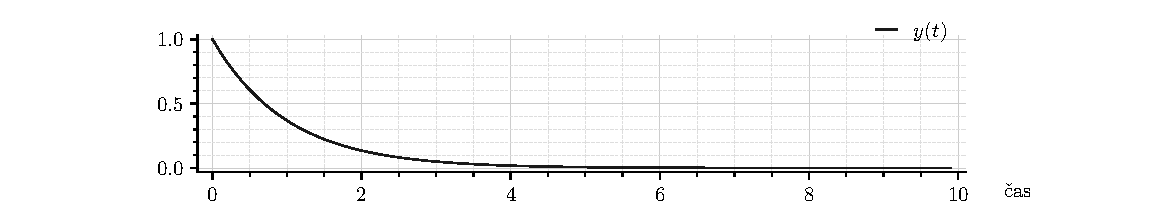
\includegraphics{ICH_SS1R_p1.pdf}
        }

        \figcaption{Impulzná charakteristika statického systému prvého rádu pre $a_0 = 1$ a $b_0 = 1$}
        \label{ICH_SS1R_p1}
    }%vbox

\end{center}

\subsubsection{ICH AS1R}

Časová funkcia \eqref{eq:ICH1R} bude impulznou charakteristikou astatického systému prvého rádu ak $a_0 = 0$. Na nasledujúcom obrázku je graf výslednej časovej funkcie

\begin{center}

    \vbox{%
        \makebox[\textwidth][c]{%
        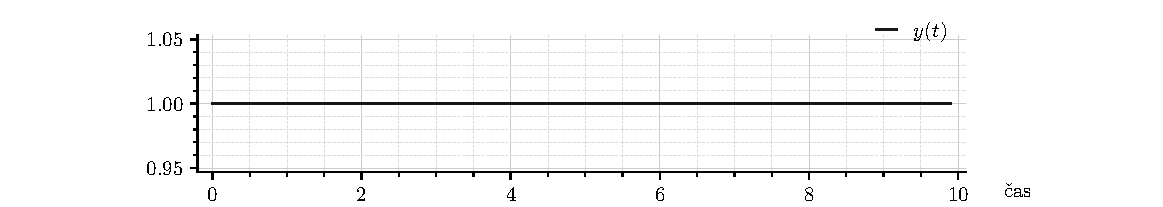
\includegraphics{ICH_AS1R_p1.pdf}
        }

        \figcaption{Impulzná charakteristika statického systému prvého rádu pre $a_0 = 0$ a $b_0 = 1$}
        \label{ICH_AS1R_p1}
    }%vbox

\end{center}





\subsubsection{ICH nestabilného systému prvého rádu}

Pre úplnosť uveďme aj prípad, keď $a_0 < 0$, teda systém je nestabilný. Zvoľme $a_0 = -1$. Na nasledujúcom obrázku je graf výslednej časovej funkcie

\begin{center}

    \vbox{%
        \makebox[\textwidth][c]{%
        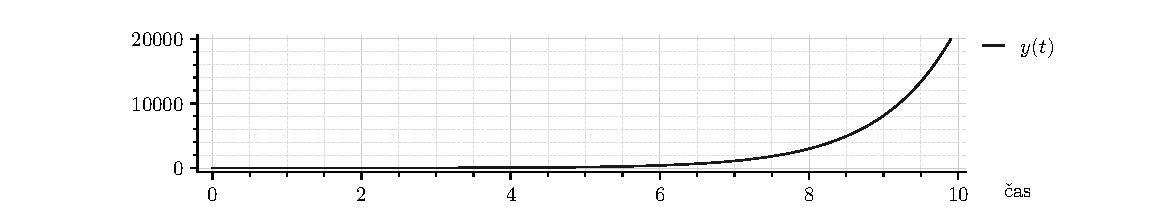
\includegraphics{ICH_unstable1R_p1.pdf}
        }

        \figcaption{Impulzná charakteristika statického systému prvého rádu pre $a_0 = -1$ a $b_0 = 1$}
        \label{ICH_unstable1R_p1}
    }%vbox

\end{center}


\subsubsection{Python skript pre vykreslenie grafov impulzných charakteristík}

V tejto časti je prezentovaný skript v programovacom jazyku Python, pomocou ktorého je možné nakresliť vyššie uvedené grafy impulzných charakteristík. Skript je prezentovaný formou Jupyter notebooku a v nasledujúcom sú zobrazené jednotlivé bunky bunky notebooku.

\input{../../PY/jupynotex/tex/MRS10_ICH1Ripynb_2-.tex}



\subsubsection{MATLAB: Control System Toolbox}

S využitím \emph{Control System Toolbox} v MATLABe je možné získať ICH príkazom  \lstinline|impulse()|. Samozrejme, najprv je potrebné zadefinovať systém, ktorého ICH nás zaujíma, čo je možné v tomto toolboxe priamo vo forme prenosovej funkcie príkazom  \lstinline|tf()|. Teda:
\begin{lstlisting}[language=Matlab,]
G = tf([1], [1, 1])
impulse(G)
\end{lstlisting}
\noindent
pričom príkaz \lstinline|impulse()| priamo vykreslí aj obrázok.


\subsubsection{MATLAB: Simulink}

V Simulinku je napríklad možné realizovať aproximáciu Dirackovho impulzu pomocou bloku \lstinline|Step| s nasledovným nastavením:
\begin{center}

    \makebox[\textwidth][c]{%
	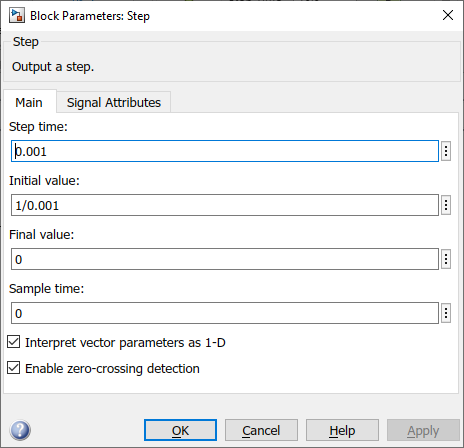
\includegraphics[width=0.68\textwidth]{stepSetup_DiracApprox.png}
	}

	\figcaption{Nastavenie bloku \lstinline|Step|.}
	\label{stepSetup_DiracApprox.png}

\end{center}

Blok je súčasťou schémy:
\begin{center}

    \makebox[\textwidth][c]{%
	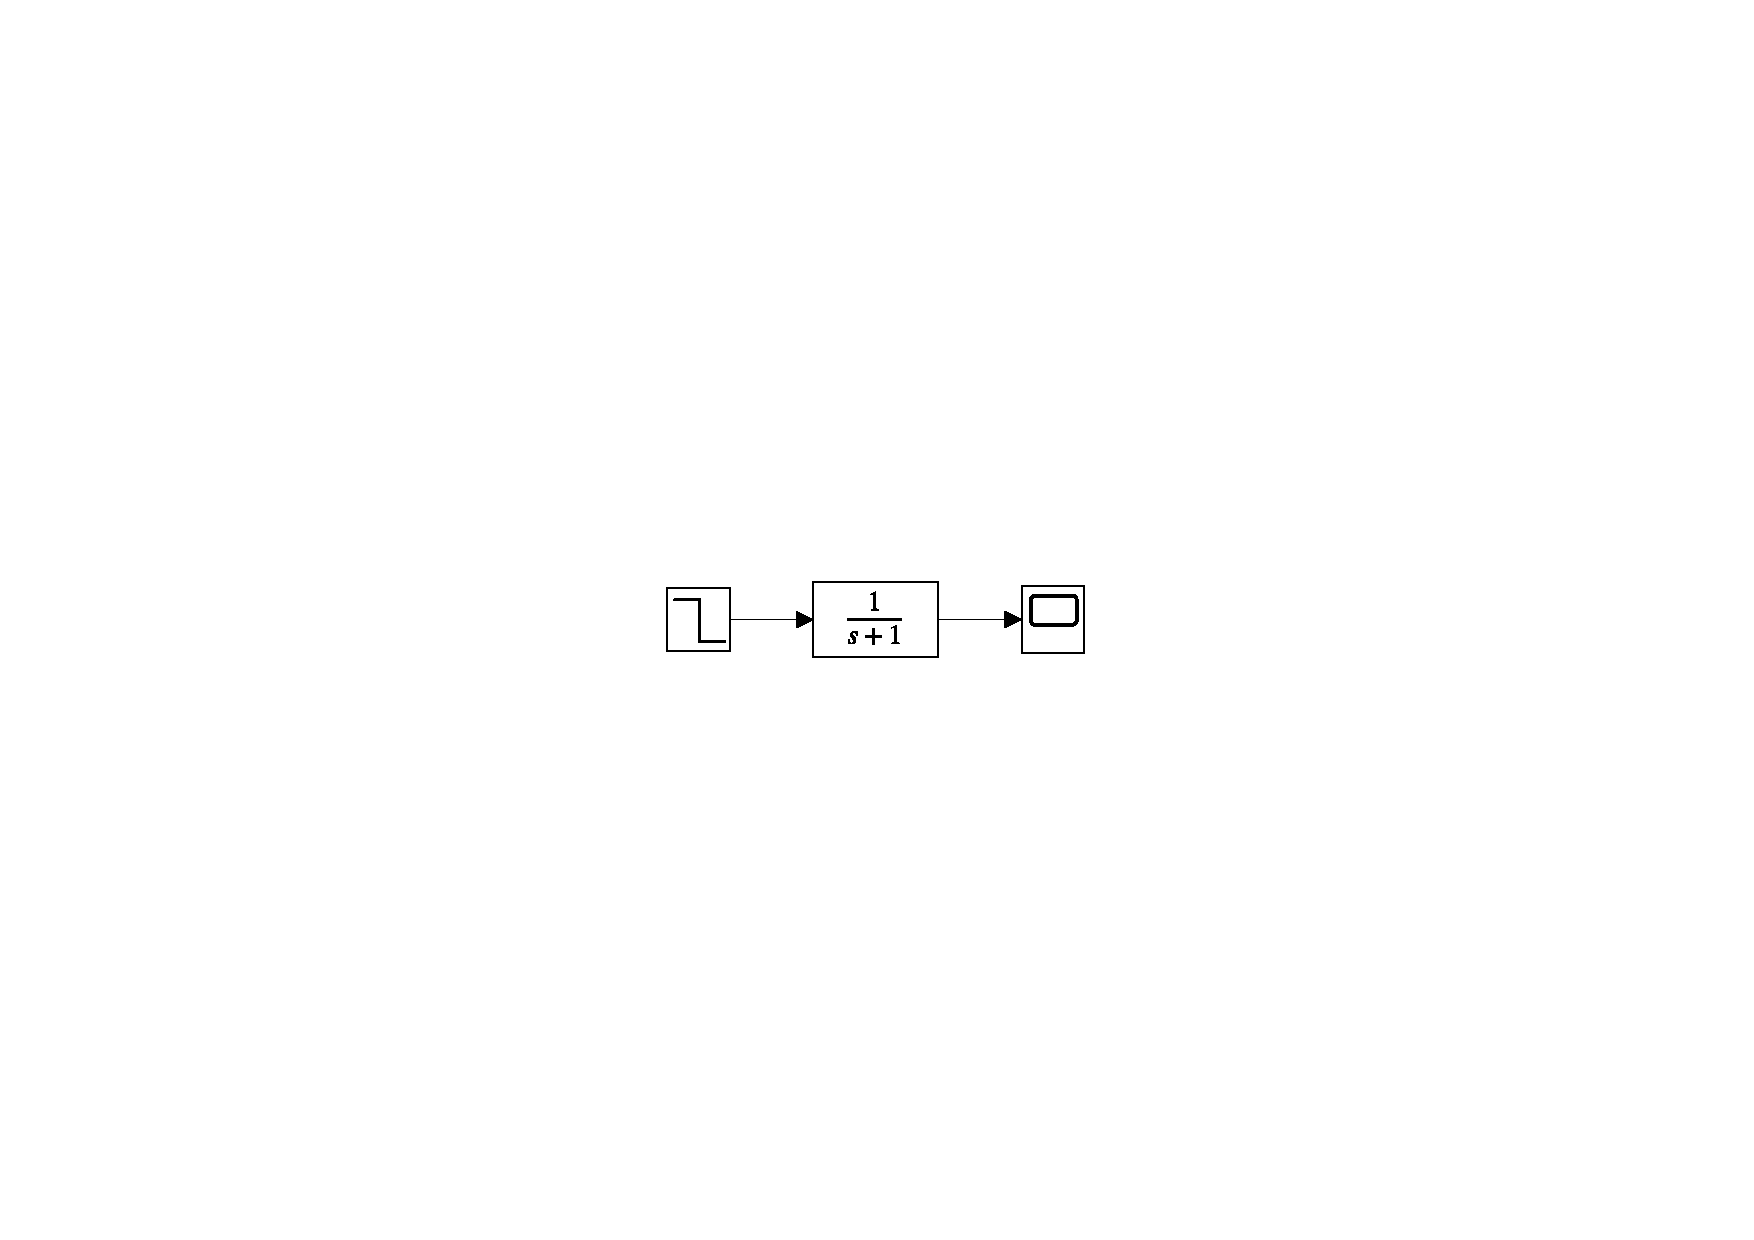
\includegraphics[trim=110mm 95mm 110mm 95mm, clip]{simulinkICHSS1R.pdf}
	}

    \vspace{-5mm}

	\figcaption{Simulačná schéma pre ICH SS1R}
	\label{sim_ICHSS1R}

    \vspace{-1mm}

\end{center}














\subsection{Prechodová charakteristika}


Prechodová charakteristika je odpoveď systému na jednotkový skok.

\bigskip

Jednotkový skok je signál, ktorý je nulový pre $t < 0$ a má jednotkovú veľkosť pre $t \geq 0$. Ide o skokovú zmenu v čase $t=0$. Laplaceov obraz jednotkového skoku je $U(s) = \frac{1}{s}$.

Keďže máme k dispozícii matematický opis systému, prechodovú charakteristiku môžeme	nájsť analyticky. Prenosová funkcia systému prvého rádu je \eqref{eq:prvyradprenosovafunkcia}. Laplaceov obraz vstupného signálu je $U(s) = \frac{1}{s}$. Laplaceov obraz výstupného signálu potom bude
\begin{subequations}
\begin{align}
    Y(s) &= G(s) U(s) = \frac{b_0}{s + a_0} \frac{1}{s} \\
    Y(s) &= \frac{b_0}{s(s + a_0)}
\end{align}
\end{subequations}
Pre hľadanie originálu tohto obrazu je výhodné prepísať tento výraz na parciálny zlomok
\begin{subequations}
\begin{align}
    \frac{b_0}{s(s + a_0)} &= \frac{A}{s} + \frac{B}{s + a_0} \\
    b_0 &= A(s + a_0) + B s
\end{align}
\end{subequations}
kde $A$ a $B$ sú neznáme koeficienty. Uvedené platí pre akúkoľvek hodnotu $s$. Pre $s = 0$ dostaneme
\begin{subequations}
\begin{align}
    b_0 &= A a_0 \\
    A &= \frac{b_0}{a_0}
\end{align}
\end{subequations}
Pre $s = -a_0$ dostaneme
\begin{subequations}
\begin{align}
    b_0 &= B (-a_0) \\
    B &= -\frac{b_0}{a_0}
\end{align}
\end{subequations}
Obraz výstupného signálu je teda
\begin{equation}
    Y(s) = \frac{b_0}{a_0} \frac{1}{s} - \frac{b_0}{a_0} \frac{1}{s + a_0}
\end{equation}
a jeho originál
\begin{subequations}
\begin{align}
    y(t) &= \frac{b_0}{a_0} - \frac{b_0}{a_0} e^{-a_0 t} \\
    y(t) &= \frac{b_0}{a_0} \left(1 - e^{-a_0 t}\right)  \label{eq:PCH1Rfull}
\end{align}
\end{subequations}
čo je časová funkcia, ktorá je analytickým vyjadrením prechodovej charakteristiky systému. V uvedenom sme zjavne predpokladali, že $a_0 \neq 0$. 

Ak $a_0 = 0$, potom obraz výstupného signálu je
\begin{subequations}
\begin{align}
    Y(s) &= \frac{b_0}{s^2} \\
    Y(s) &= b_0 \frac{1}{s^2}
\end{align}
\end{subequations}
a jeho originál je
\begin{equation} \label{eq:PCH1Rint}
    y(t) = b_0 t
\end{equation}
čo je časová funkcia, ktorá je analytickým vyjadrením prechodovej charakteristiky systému ak $a_0 = 0$.


Je zrejmé, že pre prechodovú charakteristiku (PCH) je možné rozlišovať kvalitatívne rôzne prípady určené v tomto prípade jediným pólom systému. Pól systému je $s_1 = -a_0$.

V kontexte vyššie uvedeného možno rozlišovať prípady: statický systém prvého rádu (SS1R), astatický systém prvého rádu (AS1R) a nestabilný systém.



\subsubsection{PCH SS1R}

Časová funkcia \eqref{eq:PCH1Rfull} bude prechodovou charakteristikou statického systému prvého rádu ak $a_0 > 0$. Zvoľme $a_0 = 1$ a napríklad $b_0 = 1$. Na nasledujúcom obrázku je graf výslednej časovej funkcie

\begin{center}

    \vbox{%
        \makebox[\textwidth][c]{%
        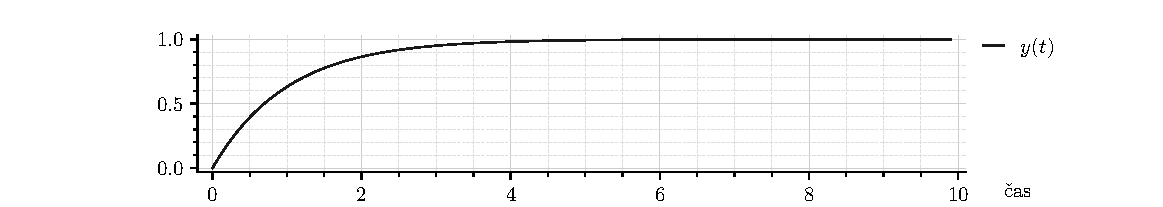
\includegraphics{PCH_SS1R_p1.pdf}
        }

        \figcaption{Prechodová charakteristika statického systému prvého rádu pre $a_0 = 1$ a $b_0 = 1$}
        \label{PCH_SS1R_p1}
    }%vbox

\end{center}



\subsubsection{PCH AS1R}

Časová funkcia \eqref{eq:PCH1Rint} bude prechodovou charakteristikou astatického systému prvého rádu ak $a_0 = 0$. Na nasledujúcom obrázku je graf výslednej časovej funkcie

\begin{center}

    \vbox{%
        \makebox[\textwidth][c]{%
        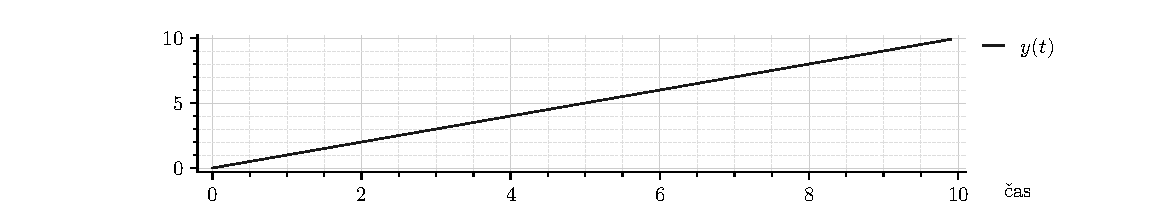
\includegraphics{PCH_AS1R_p1.pdf}
        }

        \figcaption{Prechodová charakteristika statického systému prvého rádu pre $a_0 = 0$ a~$b_0 = 1$}
        \label{PCH_AS1R_p1}
    }%vbox

\end{center}


\subsubsection{PCH nestabilného systému prvého rádu}

Pre úplnosť uveďme aj prípad, keď $a_0 < 0$, teda systém je nestabilný. Zvoľme $a_0 = -1$. Na nasledujúcom obrázku je graf výslednej časovej funkcie

\begin{center}

    \vbox{%
        \makebox[\textwidth][c]{%
        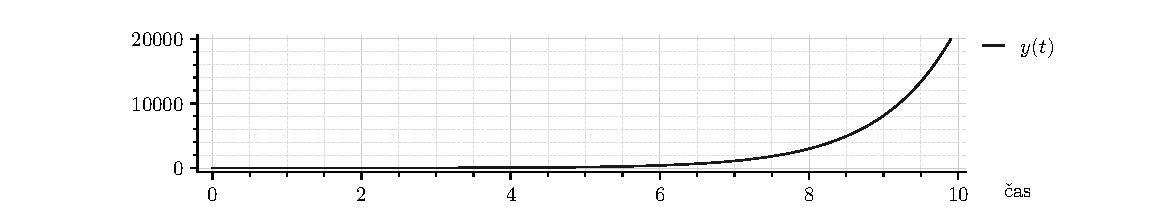
\includegraphics{PCH_unstable1R_p1.pdf}
        }

        \figcaption{Prechodová charakteristika statického systému prvého rádu pre $a_0 = -1$ a~$b_0 = 1$}
        \label{PCH_unstable1R_p1}
    }%vbox

\end{center}


\subsubsection{Python skript pre vykreslenie grafov prechodových charakteristík}

V tejto časti je prezentovaný skript v programovacom jazyku Python, pomocou ktorého je možné nakresliť vyššie uvedené grafy prechodových charakteristík. Skript je prezentovaný formou Jupyter notebooku a v nasledujúcom sú zobrazené jednotlivé bunky notebooku.


\input{../../PY/jupynotex/tex/MRS10_PCH1Ripynb_2-.tex}


\subsubsection{MATLAB: Control System Toolbox}

S využitím \emph{Control System Toolbox} v MATLABe je možné získať PCH príkazom  \lstinline|step()|. Samozrejme, najprv je potrebné zadefinovať systém, ktorého PCH nás zaujíma, čo je možné v tomto toolboxe priamo vo forme prenosovej funkcie príkazom  \lstinline|tf()|. Teda:
\begin{lstlisting}[language=Matlab,]
G = tf([1], [1, 1])
step(G)
\end{lstlisting}
\noindent
pričom príkaz \lstinline|step()| sa postará o časové nastavenie simulácie (nájde vhodné nastavenie pre ODE solver atď) a priamo vykreslí aj obrázok.


\subsubsection{MATLAB: Simulink}

Simulink priamo ponúka prácu s prenosovými funkciami a teda za užívateľa vykoná prevod do opisu v stavovom priestore a vykoná numerickú simuláciu. Pre tento prípad by schéma v simulinku vyzerala nasledovne:

\begin{center}

    \makebox[\textwidth][c]{%
	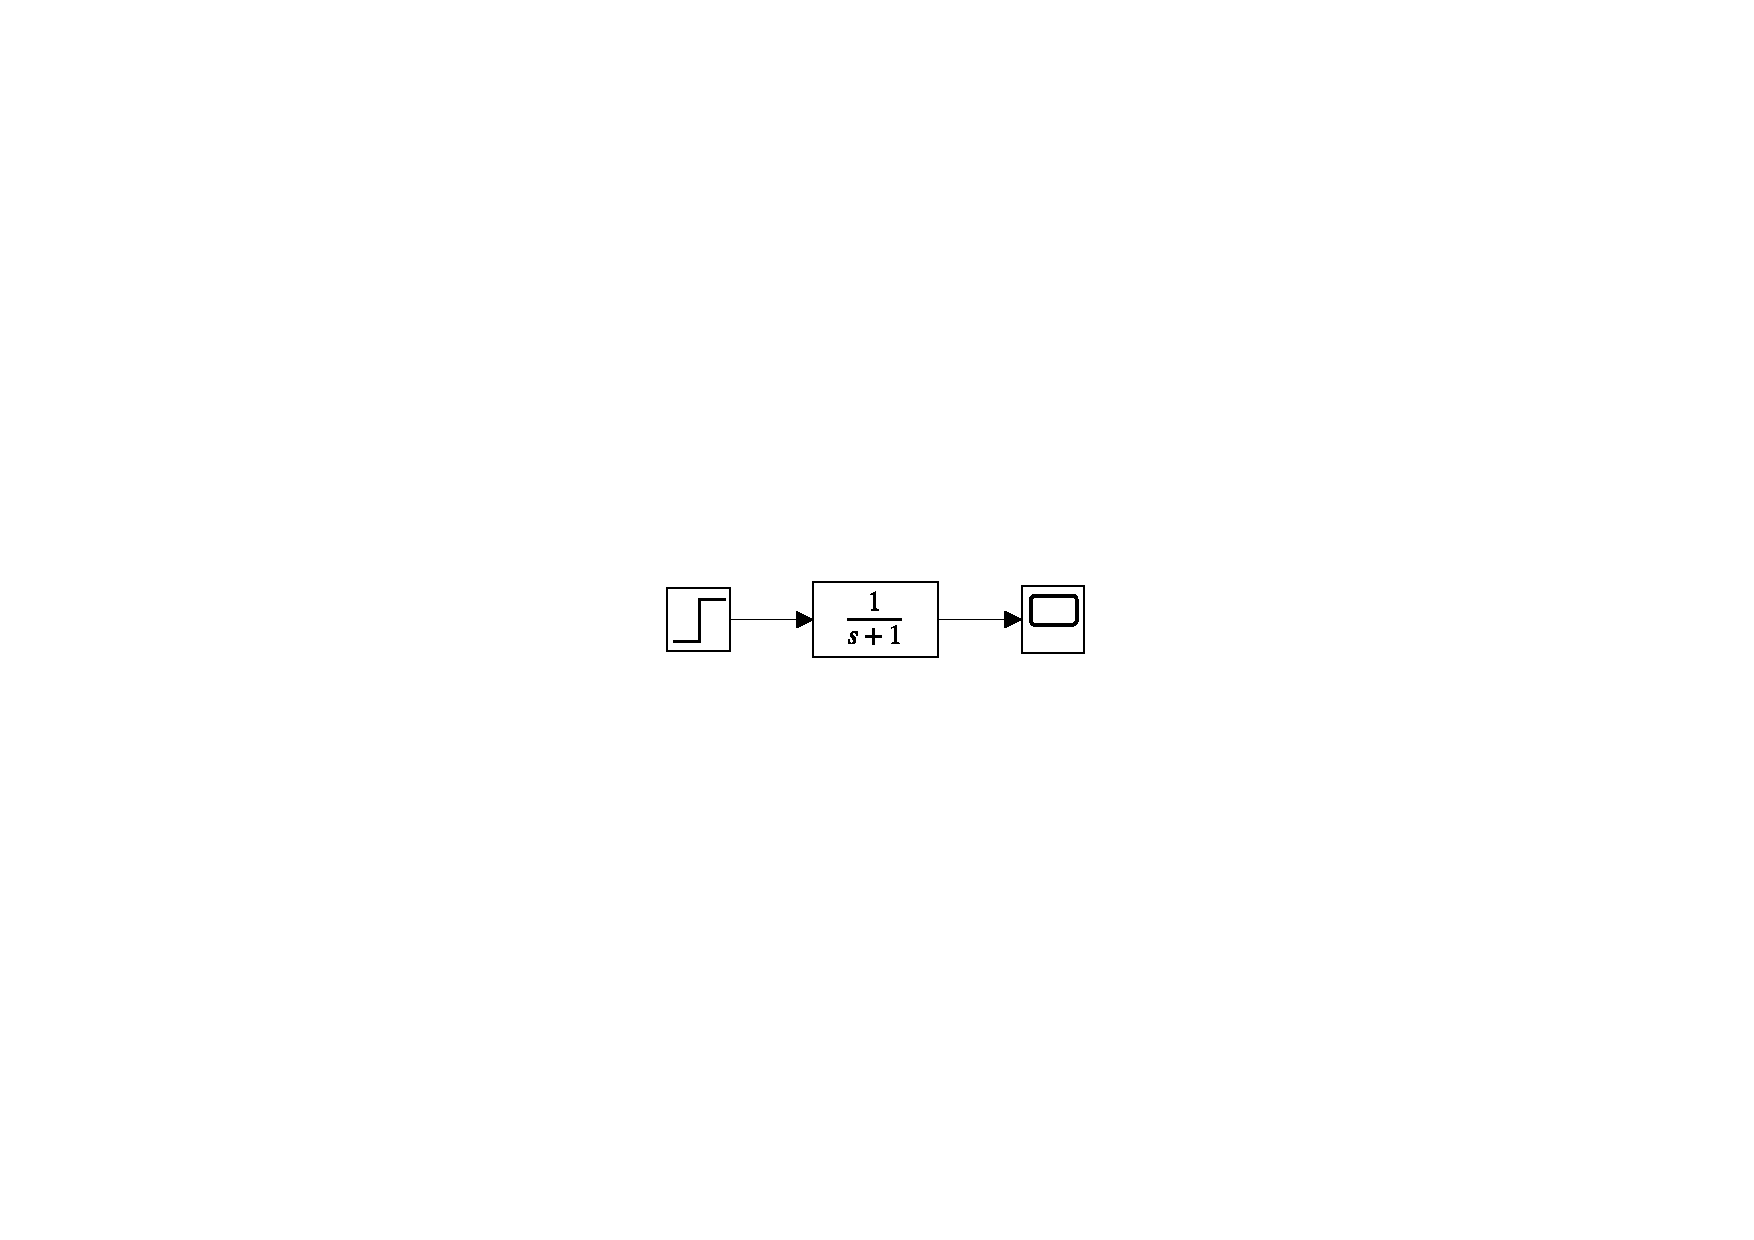
\includegraphics[trim=110mm 95mm 110mm 95mm, clip]{simulinkPCHSS1R.pdf}
	}

    \vspace{-5mm}

	\figcaption{Simulačná schéma pre PCH SS1R}
	\label{sim_PCHSS1R}

    \vspace{-1mm}

\end{center}

V bloku \lstinline|Step| je v tomto prípade nastavený skok v~čase $0$~z~hodnoty $0$~na hodnotu~$1$.

























\section{Systém nultého rádu}

Stupeň polynómu $A(s)$ môže byť aj $n = 0$. Potom hovoríme o systéme nultého rádu. Prenosová funkcia v tomto prípade je (aj vzhľadom na kauzálnosť, aj vzhľadom na pozitívnu reálnosť)
\begin{align}
    G(s) = \frac{b_0}{a_0}
\end{align}

Hovoriť v tomto prípade o dynamike v podstate nie je možné. Ide tu vo všeobecnosti o zosilňovač, ktorého statické zosilnenie je
\begin{align}
    \frac{y(\infty)}{u(\infty)} = \frac{b_0 }{a_0}
\end{align}
Takýto systém má len statické vlastnosti (statické zosilnenie -- sklon prevodovej charakteristiky). O~dynamických vlastnostiach, v~zmysle astatizmu, stability a~prechodovej charakteristiky tu nemá význam hovoriť.














\section{Systém druhého rádu}


\subsection{Prenosová funkcia}

Ak stupeň polynómu $A(s)$ je $n = 2$, potom hovoríme, že systém je druhého rádu. Pre kauzálnosť a aj pre pozitívnu reálnosť tu uvažujeme $m<n$ a tak vo všeobecnosti
\begin{align} \label{typ2radtf}
    G(s) = \frac{b_1 s + b_0}{s^2 + a_1 s + a_0}
\end{align}
kde je $A(s)$ bez straty na všeobecnosti uvedený ako monický polynóm.

Obdobne, prenosovou funkciou druhého rádu sú:
\begin{subequations}
    \begin{align}
        G(s) &= \frac{b_0}{s^2 + a_1 s + a_0} \\
        G(s) &= \frac{b_1 s}{s^2 + a_1 s + a_0}
    \end{align}
\end{subequations}



\subsection{Diferenciálna rovnica}

Nech je systém daný v tvare prenosovej funkcie
\begin{equation}
    G(s) = \frac{Y(s)}{U(s)}
\end{equation}
kde $Y(s)$ je Laplaceov obraz výstupného signálu a $U(s)$ je Laplaceov obraz vstupného signálu. Nech cieľom je prepis do tvaru diferenciálnej rovnice, potom
\begin{subequations}
    \begin{align}
        Y(s) &= G(s) U(s) = \frac{b_1 s + b_0}{s^2 + a_1 s + a_0} U(s) \\
        (s^2 + a_1 s + a_0) Y(s) &= (b_1 s + b_0) U(s) \\
        s^2 Y(s) + a_1 s Y(s) + a_0 Y(s) &= b_1 s U(s) + b_0 U(s) \\
        s^2 Y(s) &= - a_1 s Y(s) - a_0 Y(s) + b_1 s U(s) + b_0 U(s) 
    \end{align}
\end{subequations}
a teda diferenciálna rovnica je
\begin{equation} \label{difrovnica2rad}
    \ddot y(t)  =  - a_1 \dot y(t) - a_0 y(t) + b_1 \dot u(t) + b_0 u(t)
\end{equation}

Prepis opačným smerom, z dif. rovnice na prenosovú funkciu, je samozrejme štandardné aplikovanie Laplaceovej transformácie na rovnicu \eqref{difrovnica2rad} pri nulových začiatočných podmienkach.



\subsection{Opis systému v stavovom priestore}

V stavovom priestore je potrebné zaviesť stavový vektor $x(t) \in \mathbb R^n$. Vo všeobecnosti je opis lineárneho systému v stavovom priestore v tvare
\begin{subequations}
\begin{align}
    \dot x(t) &= A x(t) + b u(t) \\
    y(t) &= c^\naT x(t) 
\end{align}
\end{subequations}
kde $A \in \mathbb R^{n \times n}$, $b \in \mathbb R^n$ a $c \in \mathbb R^n$ sú matica a vektory a ide o parametre systému.

Pri stanovení vektora $x(t)$ ide vo všeobecnosti o prepis diferenciálnej rovnice vyššieho rádu na sústavu rovníc prvého rádu. Vzniknú tak nové signály, ktoré sú neznámymi v sústave rovníc prvého rádu a sú prvkami stavového vektora $x(t)$.


\subsubsection{Príkladný postup pre voľbu stavových veličín}

Prevod z prenosovej funkcie na stavový opis nie je jednoznačný. Záleží na voľbe stavových veličín (stavového priestoru). Tu si dovolíme uviesť voľbu stavových veličín tak, že výsledkom je opis systému v tzv. normálnej forme riaditeľnosti.

Prenosová funkcia systému, ktorou sa tu zaoberáme, je v tvare
\begin{align} \label{tfVseob01}
	\frac{Y(s)}{U(s)} = \frac{b_1 s + b_0}{ s^2 + a_1 s + a_0}
\end{align}
Otázka je ako túto prenosovú funkciu previesť na opis v stavovom priestore - ako zvoliť stavové veličiny.

Pre prípad, keď je v čitateli len konštanta (systém nemá nuly), je voľba stavových veličín značne intuitívna. Preto napíšme prenosovú funkciu \eqref{tfVseob01} ako dve prenosové funkcie v sérii nasledovne
\begin{align}
	\frac{Z(s)}{U(s)} &= \frac{1}{ s^2 + a_1 s + a_0} \label{tfVseob02a} \\
    \frac{Y(s)}{Z(s)} &= b_1 s + b_0 \label{tfVseob02b}
\end{align}
kde sme zaviedli pomocnú veličinu $Z(s)$, ktorá je obrazom $z(t)$. Zjavne platí
\begin{align}
    \frac{Y(s)}{U(s)} = \frac{Y(s)}{Z(s)} \frac{Z(s)}{U(s)}
\end{align}
alebo explicitnejšie:
\begin{align}
    \frac{Y(s)}{U(s)} = \left( b_1 s + b_0 \right) \frac{1}{ s^2 + a_1 s + a_0}
\end{align}

Mimochodom, prenosová funkcia \eqref{tfVseob02b} je z matematického hľadiska korektná akurát v čitateli je polynóm stupňa $1$ a v menovateli polynóm stupňa $0$, čo napríklad znamená, že ide o nekauzálny systém a teda sama o sebe by prenosová funkcia \eqref{tfVseob02b} nebola vhodným modelom reálneho fyzikálneho systému.

Prvú prenosovú funkciu \eqref{tfVseob02a} možno prepísať na diferenciálnu rovnicu druhého rádu v tvare
\begin{align} \label{origdifeqnz}
	\ddot z(t) + a_1 \dot z(t) + a_0 z(t) = u(t)
\end{align}

Túto je možné previesť na sústavu diferenciálnych rovníc prvého rádu - voľbou stavových veličín. Napríklad nech
\begin{align}
	x_1(t) = z(t)
\end{align}
kde $x_1(t)$ je prvá stavová veličina. Potom platí
\begin{align}
	\dot x_1(t) = \dot z(t)
\end{align}
Druhú stavovú veličinu zvoľme
\begin{align}
	x_2(t) = \dot z(t)
\end{align}
a teda
\begin{align} \label{zardrufdifr}
	\dot x_2(t) = \ddot z(t)
\end{align}
V tomto bode môžeme ľahko písať
\begin{align}
	\dot x_1(t) &= x_2(t)
\end{align}
To je prvá diferenciálna rovnica! Obsahuje len novo zavedené stavové veličiny ($x_1(t)$ a~$x_2(t)$). Druhá diferenciálna rovnica je vlastne \eqref{zardrufdifr}. Avšak, vieme signál $\ddot z(t)$ vyjadriť len pomocou novo zavedených stavových veličín? Vieme. Z \eqref{origdifeqnz} je zrejmé, že
\begin{align}
	\ddot z(t) = - a_1 \dot z(t) - a_0 z(t) + u(t) = - a_1 x_2(t) - a_0 x_1(t) + u(t)
\end{align}
takže \eqref{zardrufdifr} je
\begin{align}
	\dot x_2(t) =  - a_1 x_2(t) - a_0 x_1(t) + u(t)
\end{align}
a to je druhá diferenciálna rovnica\ldots

\noindent
Obe rovnice spolu:
\begin{align}
    \dot x_1(t) &= x_2(t) \\
	\dot x_2(t) &=  - a_1 x_2(t) - a_0 x_1(t) + u(t)
\end{align}
V maticovom zápise:
\begin{align}
	\begin{bmatrix}
    	  \dot x_1(t) \\
		  \dot x_2(t)
 	\end{bmatrix}
	&=
	\begin{bmatrix}
    	0 & 1 \\
    	- a_0 & - a_1
  	\end{bmatrix}
    \begin{bmatrix}
    	  x_1(t) \\
		  x_2(t)
 	\end{bmatrix}
    +
    \begin{bmatrix}
    	  0 \\
		  1
 	\end{bmatrix}
    u(t)
\end{align}

Vráťme sa k prenosovej funkcii \eqref{tfVseob02b}. Túto možno napísať ako diferenciálnu rovnicu v tvare
\begin{align} \label{difrov2}
    y(t) = b_1 \dot z(t) + b_0 z(t)
\end{align}
Avšak, my sme už urobili voľbu takú, že $\dot z(t) = x_2(t)$ a $z(t)= x_1(t)$. Takže diferenciálnu rovnicu \eqref{difrov2} môžme písať ako
\begin{align}
    y(t) = b_1 x_2(t) + b_0 x_1(t)
\end{align}
alebo v maticovom tvare
\begin{align}
	y(t)
	&=
	\begin{bmatrix}
    	b_0 & b_1 \\
  	\end{bmatrix}
    \begin{bmatrix}
    	  x_1(t) \\
		  x_2(t)
 	\end{bmatrix}
\end{align}

Celý systém s novo zavedenými stavovými veličinami teda je v tvare
\begin{align}
	\begin{bmatrix}
    	  \dot x_1(t) \\
		  \dot x_2(t)
 	\end{bmatrix}
	&=
	\begin{bmatrix}
    	0 & 1 \\
    	- a_0 & - a_1
  	\end{bmatrix}
    \begin{bmatrix}
    	  x_1(t) \\
		  x_2(t)
 	\end{bmatrix}
    +
    \begin{bmatrix}
    	  0 \\
		  1
 	\end{bmatrix}
    u(t)
    \\
    y(t)
    &=
    \begin{bmatrix}
        b_0 & b_1 \\
    \end{bmatrix}
    \begin{bmatrix}
          x_1(t) \\
          x_2(t)
    \end{bmatrix}
\end{align}
Ak označíme stavový vektor ako $x(t) = \begin{bmatrix} x_1(t) & x_2(t) \end{bmatrix}^\naT$, potom je systém v známom tvare
\begin{subequations} \label{susDifRovnicPreODE}
    \begin{align}
    	\dot x(t) &= A x(t) + b u(t) \\
        y(t) &= c^\naT x(t)
    \end{align}
\end{subequations}
kde
\begin{subequations}
\begin{align}
    A &=
    \begin{bmatrix}
    	0 & 1 \\
    	- a_0 & - a_1
  	\end{bmatrix}
    \\
    b &=
    \begin{bmatrix}
    	  0 \\
          1
 	\end{bmatrix}
    \\
    c &=
    \begin{bmatrix}
        b_0 \\ b_1 
    \end{bmatrix}
\end{align}
\end{subequations}



\subsubsection{Následné príklady priameho stanovenia opisu systému v stavovom priestore}

Vidíme, že ak máme prenosovú funkciu v tvare
\begin{align} \label{tfVseob02}
	\frac{Y(s)}{U(s)} = \frac{b_1 s + b_0}{ s^2 + a_1 s + a_0}
\end{align}
tak opis systému v stavovom priestore je v tvare
\begin{subequations}
\begin{align}
    \dot x(t)
    &=
    \begin{bmatrix}
    	0 & 1 \\
    	- a_0 & - a_1
  	\end{bmatrix}
    x(t)
    +
    \begin{bmatrix}
    	  0 \\
          1
 	\end{bmatrix}
    u(t)
    \\
    y(t)
    &=
    \begin{bmatrix}
        b_0 & b_1 \\
    \end{bmatrix}
    x(t)
\end{align}
\end{subequations}
kde samozrejme $x(t) \in \mathbb R^2$ je stavový vektor. 
Obdobne, ak máme prenosovú funkciu v~tvare
\begin{align} 
	\frac{Y(s)}{U(s)} = \frac{b_0}{ s^2 + a_1 s + a_0}
\end{align}
tak opis systému v stavovom priestore je v tvare
\begin{subequations}
\begin{align}
    \dot x(t)
    &=
    \begin{bmatrix}
    	0 & 1 \\
    	- a_0 & - a_1
  	\end{bmatrix}
    x(t)
    +
    \begin{bmatrix}
    	  0 \\
          1
 	\end{bmatrix}
    u(t)
    \\
    y(t)
    &=
    \begin{bmatrix}
        b_0 & 0 \\
    \end{bmatrix}
    x(t)
\end{align}
\end{subequations}
čo je možné zapísať aj v tvare
\begin{subequations}
    \begin{align}
        \dot x(t)
        &=
        \begin{bmatrix}
            0 & 1 \\
            - a_0 & - a_1
          \end{bmatrix}
        x(t)
        +
        \begin{bmatrix}
              0 \\
              b_0
         \end{bmatrix}
        u(t)
        \\
        y(t)
        &=
        \begin{bmatrix}
            1 & 0 \\
        \end{bmatrix}
        x(t)
\end{align}
\end{subequations}
pretože sme len zmenili miesto, kde koeficient $b_0$ násobí zodpovedajúci signál. Je jedno, či je to na vstupe, alebo na výstupe. 

Pre úplnosť, ak máme prenosovú funkciu v tvare
\begin{align} 
	\frac{Y(s)}{U(s)} = \frac{b_1 s }{ s^2 + a_1 s + a_0}
\end{align}
tak opis systému v stavovom priestore je v tvare
\begin{subequations}
\begin{align}
    \dot x(t)
    &=
    \begin{bmatrix}
    	0 & 1 \\
    	- a_0 & - a_1
  	\end{bmatrix}
    x(t)
    +
    \begin{bmatrix}
    	  0 \\
          1
 	\end{bmatrix}
    u(t)
    \\
    y(t)
    &=
    \begin{bmatrix}
        0 & b_1 \\
    \end{bmatrix}
    x(t)
\end{align}
\end{subequations}
Ešte iným príkladom by mohla byť prenosová funkcia v tvare
\begin{align} 
	\frac{Y(s)}{U(s)} = \frac{b_0 }{ s^2 +  a_0}
\end{align}
a opis systému v stavovom priestore by bol
\begin{subequations}
    \begin{align}
        \dot x(t)
        &=
        \begin{bmatrix}
            0 & 1 \\
            0 & - a_1
          \end{bmatrix}
        x(t)
        +
        \begin{bmatrix}
              0 \\
              1
         \end{bmatrix}
        u(t)
        \\
        y(t)
        &=
        \begin{bmatrix}
            b_0 & 0 \\
        \end{bmatrix}
        x(t)
\end{align}
\end{subequations}



\subsubsection{Z opisu v stavovom priestore na prenosovú funkciu}

Majme systém daný v stavovom priestore v tvare
\begin{subequations} \label{difRovSustavaKPrevodu}
    \begin{align} 
        \dot x(t) &= A x(t) + b u(t) \label{difRovSustavaKPrevodua}\\
        y(t) &= c^\naT x(t) 
    \end{align}
\end{subequations}
kde stavový vektor $x(t) \in \mathbb R^n$, $A \in \mathbb R^{n \times n}$, $b \in \mathbb R^n$ a $c \in \mathbb R^n$ sú matica a vektory a ide o parametre systému. 

Rovnica \eqref{difRovSustavaKPrevodua} je takpovediac vektorovou diferenciálnou rovnicou, čím tu myslíme, že neznámou je vektor $x(t)$ obsahujúci signály (stavové veličiny).

Na rovnice \eqref{difRovSustavaKPrevodu} je možné aplikovať Laplaceovú transformáciu. Potom pri nulových začiatočných podmienkach, pretože našim cieľom je prenosová funkcia, je možné písať
\begin{subequations}
    \begin{align}
        s I X(s) &= A X(s) + b U(s) \label{SRovSustavaKPrevodua} \\
        Y(s) &= c^\naT X(s) \label{SRovSustavaKPrevodub}
    \end{align}
\end{subequations}
kde $I$ je jednotková matica rovnakého rozmeru ako $A$ a $s$ je Laplaceov operátor. Výraz $s I$ je potom matica, ktorá má na diagonále Laplaceove operátory. $X(s)$ je samozrejme vektor, ktorý obsahuje Laplaceove obrazy stavových veličín.

Prenosová funkcia je pomerom obrazov výstupu a vstupu. Je vhodné začať rovnicou \eqref{SRovSustavaKPrevodua} a vyjadriť pomer obrazov $X(s)$ a $U(s)$. Môžeme písať
\begin{align}
    s I X(s) &= A X(s) + b U(s) \\
    s I X(s) - A X(s) &= b U(s)
\end{align}
pričom rozmery jednotlivých matíc a vektorov boli zachované. Potom
\begin{align}
    (s I - A) X(s) &= b U(s)
\end{align}
kde $(s I - A)$ je matica. Je potrebné osamostatniť $X(s)$. Celú rovnicu je preto potrebné vynásobiť zľava inverznou maticou k matici $(s I - A)$, teda maticou $(s I - A)^{-1}$.
\begin{align}
    (s I - A)^{-1} (s I - A) X(s) &= (s I - A)^{-1} b U(s) \\
    X(s) &= (s I - A)^{-1} b U(s)
\end{align}
Teraz je možné dosadiť za $X(s)$ do rovnice \eqref{SRovSustavaKPrevodub}, teda
\begin{align}
    Y(s) &= c^\naT X(s) \\
    Y(s) &= c^\naT (s I - A)^{-1} b U(s)
\end{align}
Pomer $Y(s)$ a $U(s)$ je
\begin{align}
    \frac{Y(s)}{U(s)} = c^\naT (s I - A)^{-1} b
\end{align}
a teda prenosová funkcia je
\begin{align}
    G(s) = c^\naT (s I - A)^{-1} b
\end{align}

Majme konkrétny prípad, keď systém je daný v stavovom priestore v tvare
\begin{subequations}
    \begin{align}
        \dot x(t)
        &=
        \begin{bmatrix}
            0 & 1 \\
            - a_0 & - a_1
          \end{bmatrix}
        x(t)
        +
        \begin{bmatrix}
              0 \\
              1
         \end{bmatrix}
        u(t)
        \\
        y(t)
        &=
        \begin{bmatrix}
            b_0 & b_1 \\
        \end{bmatrix}
        x(t)
\end{align}
\end{subequations}
a teda $A = \begin{bmatrix} 0 & 1 \\ - a_0 & - a_1 \end{bmatrix}$, $b = \begin{bmatrix} 0 \\ 1 \end{bmatrix}$ a $c = \begin{bmatrix} b_0 \\ b_1 \end{bmatrix}$. Stanovme maticu $(s I - A)$:
\begin{align}
    (s I - A) &=
    \begin{bmatrix}
        s & 0 \\
        0 & s
    \end{bmatrix}
    -
    \begin{bmatrix}
        0 & 1 \\
        - a_0 & - a_1
    \end{bmatrix}
    =
    \begin{bmatrix}
        s & -1 \\
        a_0 & s + a_1
    \end{bmatrix}
\end{align}
Jej inverzia je
\begin{align}
\begin{aligned}
    (s I - A)^{-1} &=
    \begin{bmatrix}
        s & -1 \\
        a_0 & s + a_1
    \end{bmatrix}^{-1}
    =
    \frac{1}{(s + a_1)s - (-a_0)}
    \begin{bmatrix}
        s + a_1 & 1 \\
        -a_0 & s
    \end{bmatrix} \\
    &=
    \frac{1}{s^2 + a_1s + a_0}
    \begin{bmatrix}
        s + a_1 & 1 \\
        -a_0 & s
    \end{bmatrix} \\
    &=
    \begin{bmatrix}
        \frac{s + a_1}{s^2 + a_1s + a_0} & \frac{1}{s^2 + a_1s + a_0} \\
        \frac{-a_0}{s^2 + a_1s + a_0} & \frac{s}{s^2 + a_1s + a_0}
    \end{bmatrix}
\end{aligned}
\end{align}
Vynásobme sprava vektorom $b$
\begin{align}
    (s I - A)^{-1} b &=
    \begin{bmatrix}
        \frac{s + a_1}{s^2 + a_1s + a_0} & \frac{1}{s^2 + a_1s + a_0} \\
        \frac{-a_0}{s^2 + a_1s + a_0} & \frac{s}{s^2 + a_1s + a_0}
    \end{bmatrix}
    \begin{bmatrix}
        0 \\ 1
    \end{bmatrix}
    =
    \begin{bmatrix}
        \frac{1}{s^2 + a_1s + a_0} \\
        \frac{s}{s^2 + a_1s + a_0}
    \end{bmatrix}
\end{align}
a následne zľava vektorom $c^\naT$
\begin{align}
    c^\naT (s I - A)^{-1} b &=
    \begin{bmatrix}
        b_0 & b_1
    \end{bmatrix}
    \begin{bmatrix}
        \frac{1}{s^2 + a_1s + a_0} \\
        \frac{s}{s^2 + a_1s + a_0}
    \end{bmatrix}
    =
    b_0 \frac{1}{s^2 + a_1s + a_0} + b_1 \frac{s}{s^2 + a_1s + a_0}
\end{align}
a po úprave
\begin{align}
    c^\naT (s I - A)^{-1} b &=
    \frac{b_0 + b_1 s}{s^2 + a_1s + a_0} 
\end{align}
je prenosová funkcia v konkrétnom uvažovanom prípade.





\subsubsection{Z opisu v stavovom priestore na diferenciálnu rovnicu}

Majme systém daný v stavovom priestore v tvare
\begin{align}
	\begin{bmatrix}
    	  \dot x_1(t) \\
		  \dot x_2(t)
 	\end{bmatrix}
	&=
	\begin{bmatrix}
    	0 & 1 \\
    	- a_0 & - a_1
  	\end{bmatrix}
    \begin{bmatrix}
    	  x_1(t) \\
		  x_2(t)
 	\end{bmatrix}
    +
    \begin{bmatrix}
    	  0 \\
		  1
 	\end{bmatrix}
    u(t)
    \\
    y(t)
    &=
    \begin{bmatrix}
        b_0 & b_1 \\
    \end{bmatrix}
    \begin{bmatrix}
          x_1(t) \\
          x_2(t)
    \end{bmatrix}
\end{align}
Nech cieľ je prepísať túto sústavu diferenciálnych rovníc na jednu sústavu rovníc vyššieho rádu. V takom prípade je možné pozerať sa na výstupný signál $y(t)$ ako na neznámu v dif. rovnici vyššieho rádu. Sústava rovníc vyzerá nasledovne:
\begin{align}
    \dot x_1(t) &= x_2(t) \label{pr_prva}\\
    \dot x_2(t) &= - a_1 x_2(t) - a_0 x_1(t) + u(t) \label{pr_druha}\\
    y(t) &= b_0 x_1(t) + b_1 x_2(t) \label{pr_tretia}
\end{align}
Napríklad rovnicu \eqref{pr_druha} zderivujme a dosaďme za $\dot x_1(t)$ z prvej rovnice \eqref{pr_prva}
\begin{align}
    \ddot x_2(t) &= - a_1 \dot x_2(t) - a_0 \dot x_1(t) + \dot u(t) \\
    \ddot x_2(t) &= - a_1 \dot x_2(t) - a_0 x_2(t) + \dot u(t) \label{92}
\end{align}
Z rovnice \eqref{pr_tretia} plynie
\begin{align}
    x_2(t) &= \frac{1}{b_1} y(t)  + \frac{b_0}{b_1}  x_1(t) \label{93} \\
    \dot x_2(t) &= \frac{1}{b_1} \dot y(t)  + \frac{b_0}{b_1}  \dot x_1(t) = \frac{1}{b_1} \dot y(t) + \frac{b_0}{b_1}  x_2(t)  \label{94}
\end{align}
a
\begin{subequations} \label{95}
    \begin{align}
        \ddot x_2(t) &= \frac{1}{b_1} \ddot y(t) + \frac{b_0}{b_1} \dot x_2(t) \\
        &= \frac{1}{b_1} \ddot y(t) + \frac{b_0}{b_1} \left( - a_1 x_2(t) - a_0 x_1(t) + u(t) \right) \\
        &= \frac{1}{b_1} \ddot y(t) - \frac{b_0 a_1}{b_1} x_2(t) - \frac{b_0 a_0}{b_1} x_1(t) + \frac{b_0}{b_1} u(t)
    \end{align} 
\end{subequations}
Výsledky \eqref{93} a \eqref{94} a \eqref{95} je možné dosadiť do \eqref{92}, teda
\begin{align}
    &
    \begin{aligned}
    & 
    \frac{1}{b_1} \ddot y(t) - \frac{b_0 a_1}{b_1} x_2(t) - \frac{b_0 a_0}{b_1} x_1(t) + \frac{b_0}{b_1} u(t) 
    \\&
    = - a_0 \left( \frac{1}{b_1} y(t)  + \frac{b_0}{b_1}  x_1(t) \right) - a_1 \left( \frac{1}{b_1} \dot y(t) + \frac{b_0}{b_1}  x_2(t) \right) + \dot u 
    \end{aligned} \\
    &
    \begin{aligned}
    &
    \frac{1}{b_1} \ddot y(t) - \frac{b_0 a_1}{b_1} x_2(t) - \frac{b_0 a_0}{b_1} x_1(t) + \frac{b_0}{b_1} u(t)
    \\&
    = -  \frac{a_0}{b_1}  y(t) -  \frac{ a_0 b_0}{b_1}  x_1(t) -  \frac{a_1}{b_1} \dot y(t) -  \frac{a_1 b_0}{b_1}  x_2(t) + \dot u
    \end{aligned}
\end{align}
a teda
\begin{align}
    \frac{1}{b_1} \ddot y(t)  + \frac{b_0}{b_1} u(t) &= -  \frac{a_0}{b_1}  y(t)  -  \frac{a_1}{b_1} \dot y(t)  + \dot u \\
    \ddot y(t)  + b_0 u(t) &= -  a_0 y(t)  -  a_1 \dot y(t)  + b_1 \dot u \\
    \ddot y(t)  &= -  a_1 \dot y(t)  -  a_0 y(t)  + b_1 \dot u(t) + b_0 u(t)
\end{align}





\subsection{Stabilita}

Stabilita systému je daná koreňmi charakteristického polynómu $A(s)$, v tomto prípade
\begin{align}
    A(s) = s^2 + a_1 s + a_0
\end{align}
Tento polynóm má dva korene. Môžu to byť:
\begin{itemize}[leftmargin=0pt, labelsep=3mm, itemsep=0pt]
    \item dve rôzne reálne čísla (imaginárna časť čísla je nulová),
    \item jedno reálne číslo, ktoré je dvojnásobným koreňom,
    \item alebo dve komplexné čísla, ktoré sú však navzájom komplexne združené.
\end{itemize}
V každom prípade však platí, že systém je stabilný vtedy, a len vtedy, ak reálne časti pólov sú záporné (v ľavej polrovine komplexnej roviny).

Ak aspoň jeden koreň leží na imaginárnej osi (reálna časť koreňa je nulová), potom hovoríme, že systém je na hranici stability.

Ak aspoň jeden koreň má reálnu časť kladnú, potom je systém nestabilný.



\subsection{Statické zosilnenie a astatizmus}

\subsubsection{Statické zosilnenie}

Uvažujme systém, ktorý nie je nestabilný a žiadny z pólov systému nie je nulový. Takýto systém je možné nazvať statickým, pretože pri ustálenom vstupe sa ustáli aj výstup. V tomto prípade máme systém druhého rádu a teda hovoríme o \emph{statickom systéme druhého ráu}, skratka SS2R. 

Pre takýto systém je možné určiť jeho statické zosilnenie. Statické zosilnenie je pomer výstupu ku vstupu v ustálenom stave.

V ustálenom stave sa signály nemenia, to znamená, že ich časové derivácie sú nulové. Všimnime si diferenciálnu rovnicu \eqref{difrovnica2rad}. 
V ustálenom stave je $\dot y(\infty) = 0$, kde $\infty$ symbolizuje čas, v ktorom sú už signály ustálené. Rovnako aj $\ddot y(\infty) = 0$ a $\dot u(\infty) = 0$ a teda
\begin{equation}
    0 = -a_0 y(\infty) + b_0 u(\infty)
\end{equation}
Pomer výstupu ku vstupu je
\begin{equation}
    \frac{y(\infty)}{u(\infty)} = \frac{b_0}{a_0}
\end{equation}
čo je statické zosilnenie systému. Túto hodnotu je možné označiť ako samostatný parameter systému, napr. $K = \frac{b_0}{a_0}$.


Konvenciou je tiež vo všeobecnosti uvažovať, že vstup je „jednotkový“, jednoducho, že $u(\infty) = 1$ a teda sa píše $y(\infty) = \frac{b_0 }{a_0}$. K rovnakému záveru prídeme, ak by sme uvažovali konštantný, ustálený signál na vstupe, a to vo všeobecnosti, teda $u(t) = 1$. To je jednotkový skok a teda $U(s) = \frac{1}{s}$. Potom
\begin{align}
    Y(s) = \frac{b_1 s + b_0}{s^2 + a_1 s + a_0} \frac{1}{s}
\end{align}
Konečná hodnota tohto obrazu signálu ($Y(s)$ je obrazom $y(t)$), je hodnota na, ktorej sa výstup systému potenciálne ustáli. S využitím vety o konečnej hodnote:
\begin{subequations}
    \begin{align}
        y(\infty) &= \lim_{s \to 0} s Y(s) \\
        &= \lim_{s \to 0} s \frac{b_1 s + b_0}{s^2 + a_1 s + a_0} \frac{1}{s} \\
        &= \lim_{s \to 0} \frac{b_1 s + b_0}{s^2 + a_1 s + a_0} \\
        &= \frac{b_0}{a_0}
    \end{align}
\end{subequations}



\subsubsection{Astatizmus}

Ak je jeden z pólov systému nulový, hovoríme, že systém je astatický („obsahuje astatizmus“). Ak práve jeden pól je nulový, hovoríme o astatizme prvého rádu. Ak sú dva póly nulové, potom ide o astatizmus druhého rádu, atď.

V tomto prípade je systém druhého rádu a teda hovoríme o \emph{astatickom systéme druhého rádu}, skratka AS2R.

V tomto prípade máme dva póly (úplne vo všeobecnosti ide o dve komplexné čísla). Póly označme $p_1$ a $p_2$. Ak je jeden z nich nulový, $p_1 = 0$, potom
\begin{align}
    A(s) = (s - p_1)(s - p_2) = (s -0)(s - p_2) = s(s - p_2)
\end{align}
Prenosová funkcia systému druhého rádu s astatizmom prvého rádu by teda mohla byť v tvare
\begin{subequations}
    \begin{align}
        G(s) &= \frac{b_1 s + b_0}{s(s - p_2)} \\
        G(s) &= \frac{b_0}{s(s - p_2)}
        % G(s) &= \frac{b_1 s}{s(s - p_2)}
    \end{align}
\end{subequations}
Všimnime si, že ak by $G(s) = \frac{b_1 s}{s(s - p_2)}$ potom je to vlastne $G(s) = \frac{b_1}{(s - p_2)}$, a~teda nejde o~systém druhého rádu\footnote{Krátime tu vo všeobecnosti polynómy a je potrebné to zohľadniť z matematického hľadiska („deliť polynómom“ nie je vždy možné)}.

Ak by boli oba póly nulové, teda $A(s) = s^2$, potom prenosová funkcia systému druhého rádu s astatizmom druhého rádu by mohla byť v tvare
\begin{subequations}
    \begin{align}
        G(s) &= \frac{b_1 s + b_0}{s^2} \\
        G(s) &= \frac{b_0}{s^2} \label{integratordvojitz}
    \end{align}
\end{subequations}

Mimochodom, prenosová funkcia \eqref{integratordvojitz} je vlastne dvojitý integrátor.




\subsection{Prevodová charakteristika}

V prípade lineárnych systémov je prevodová charakteristika priamka a bez straty na všeobecnosti môžeme uvažovať, že prechádza začiatkom súradnicového systému. Sklon priamky je daný statickým zosilnením systému, ak použijeme vyššie uvedené, sklon prevodovej charakteristiky lineárneho systému je $K = \frac{b_0}{a_0}$.


\subsection{Impulzná charakteristika}

Impulzná charakteristika je odpoveď systému na Dirackov impulz.

Keďže máme k dispozícii matematický opis systému, impulznú charakteristiku môžeme nájsť analyticky. Laplaceov obraz Dirackovho impulzu je $U(s) = 1$.


\subsubsection{ICH SS2R, prípad $B(s) = b_0$}

V prvom rade uvažujme prípad, keď dynamiku systému určujú len póly systému, teda prenosová funkcia je v tvare
\begin{align}
    G(s) =  \frac{b_0}{s^2 + a_1 s + a_0}
\end{align}

Polynóm $B(s) = b_0$ je nultého stupňa, teda systém nemá žiadne nuly. Označme póly systému $p_1$ a $p_2$. 



\paragraph{Dva nezávislé reálne póly}

Zvoľme prípad, keď sú dva nezávislé reálne póly, teda napr. $p_1 = -1$ a $p_2 = -2$. Parameter $b_0$ zvoľme tak, že statické zosilnenie systému bude jednotkové, teda $b_0 = a_0$. 

Polynóm $A(s)$ je teda $A(s) = \left( s + 1 \right) \left( s + 2 \right) = s^2 + 3s + 2$ a~parameter $b_0 = 2$. Obraz výstupnej veličiny pri Dirackovom impulze na vstupe teda je
\begin{align}
    Y(s) = \frac{2}{s^2 + 3s + 2} = \frac{2}{(s + 1)(s + 2)} = \frac{2}{s + 1} - \frac{2}{s + 2}
\end{align}
originál potom je
\begin{align} \label{fun_ICH_SS2R_v1}
    y(t) = 2e^{-t} - 2e^{-2t}
\end{align}
\begin{center}

    \vbox{%
        \makebox[\textwidth][c]{%
        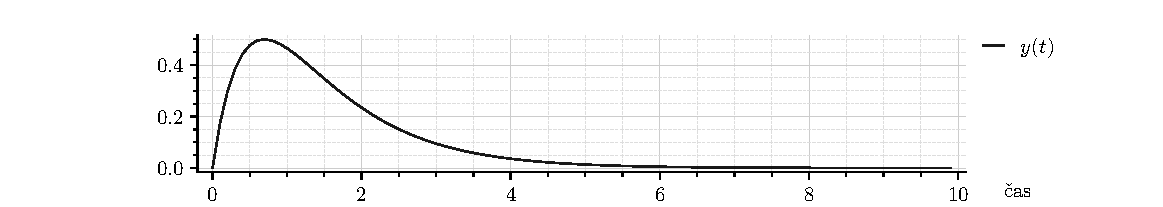
\includegraphics{ICH_SS2R_v1_p1.pdf}
        }

        \figcaption{Graf funkcie \eqref{fun_ICH_SS2R_v1}}
        \label{ICH_SS2R_v1_p1}
    }%vbox

\end{center}
Overme v MATLAB-e pomocou \lstinline|Symbolic Math Toolbox| a pomocou \lstinline|Control System Toolbox|:

% python .\jupynotex.py ..\MRS10_ICH2R_ML.ipynb '1-2' '70'

\input{../../PY/jupynotex/tex/MRS10_ICH2R_MLipynb_1-2.tex}




\paragraph{Dva rovnaké reálne póly (jeden dvojnásobný pól)}

Zvoľme prípad, keď sú dva nezávislé reálne póly, teda napr. $p_1 = -1$ a $p_2 = -1$. Parameter $b_0$ zvoľme tak, že statické zosilnenie systému bude jednotkové, teda $b_0 = a_0$. 

Polynóm $A(s)$ je teda $A(s) = \left( s + 1 \right) \left( s + 1 \right) = s^2 + 2s + 1$ a~parameter $b_0 = 1$. Obraz výstupnej veličiny pri Dirackovom impulze na vstupe teda je
\begin{align}
    Y(s) = \frac{1}{s^2 + 2s + 1} = \frac{1}{(s + 1)(s + 1)} = \frac{1}{\left(s+1\right)^2}
\end{align}
Originál potom je
\begin{align} \label{fun_ICH_SS2R_v2}
    y(t) = te^{-t}  
\end{align}
\begin{center}

    \vbox{%
        \makebox[\textwidth][c]{%
        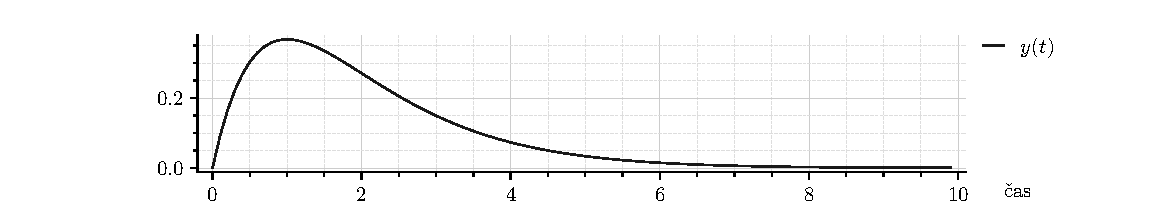
\includegraphics{ICH_SS2R_v2_p1.pdf}
        }

        \figcaption{Graf funkcie \eqref{fun_ICH_SS2R_v2}}
        \label{ICH_SS2R_v2_p1}
    }%vbox

\end{center}




\paragraph{Dva komplexne združené póly}

Ak by sme chceli póly systému, ktoré sú navzájom komplexne združenými číslami, potom je v prípade systému druhého rádu výhodné uvažovať charakteristický polynóm v tvare
\begin{align}
    A(s) = s^2 + 2 \beta \omega_0 s + \omega_0^2
\end{align}
kde $\beta$ a $\omega_0$ sú parametre, pričom $\beta$ sa nazýva koeficient tlmenia a $\omega_0$ sa nazýva vlastná frekvencia systému. Uvedené označovanie a forma polynómu $A(s)$ vyplývajú z konvencií pri opise oscilácií ako dynamického deja (diferenciálne rovnice tlmených oscilátorov). Ak je parameter $\beta < 1$, potom korene $A(s)$ sú komplexne združené čísla. Ak je parameter $\beta \geq 1$, potom korene $A(s)$ sú reálne.

Zvoľme $\beta = 0,5$ a $\omega_0 = 3$. Polynóm $A(s)$ je teda $A(s) = s^2 + 3s + 9 = \left( s + \frac{3}{2} + \frac{3}{2} \sqrt{3} j \right) \left( s + \frac{3}{2} - \frac{3}{2} \sqrt{3} j \right) $. Parameter $b_0$ zvoľme tak, že statické zosilnenie systému bude jednotkové, teda $b_0 = 9$. Obraz výstupnej veličiny pri Dirackovom impulze na vstupe teda je
\begin{align}
    \begin{aligned}
        Y(s) &= \frac{9}{s^2 + 3s + 9} \\
        &= \frac{9}{\left( s + \frac{3}{2} + \frac{3}{2} \sqrt{3} j \right) \left( s + \frac{3}{2} - \frac{3}{2} \sqrt{3} j \right)} \\
        &= \frac{A}{s + \frac{3}{2} + \frac{3}{2} \sqrt{3} j} + \frac{B}{s + \frac{3}{2} - \frac{3}{2} \sqrt{3} j}
    \end{aligned}
\end{align}
kde $A$ a $B$ sú konštanty, ktoré je potrebné nájsť. Platí
\begin{align}
    9 = A \left( s + \frac{3}{2} - \frac{3}{2} \sqrt{3} j \right) + B \left( s + \frac{3}{2} + \frac{3}{2} \sqrt{3} j \right)
\end{align}
Pre $s = - \frac{3}{2} - \frac{3}{2} \sqrt{3} j$ potom
\begin{align}
    \begin{aligned}
        9 &= A \left( - \frac{3}{2} - \frac{3}{2} \sqrt{3} j + \frac{3}{2} - \frac{3}{2} \sqrt{3} j \right) \\
        &= A \left( - 3 \sqrt{3} j   \right) 
    \end{aligned} 
\end{align}
\begin{align}    
        A &= \frac{9}{- 3 \sqrt{3} j} = \frac{3}{-  \sqrt{3} j} \cdot \frac{\sqrt{3} j}{\sqrt{3} j} = \frac{3 \sqrt{3} j}{3} = \sqrt{3} j
\end{align}
Pre $s = - \frac{3}{2} + \frac{3}{2} \sqrt{3} j$ potom
\begin{align}
    \begin{aligned}
        9 &= B \left( - \frac{3}{2} + \frac{3}{2} \sqrt{3} j + \frac{3}{2} + \frac{3}{2} \sqrt{3} j \right) \\
        &= B \left(  3 \sqrt{3} j   \right) 
    \end{aligned} 
\end{align}
\begin{align}    
    B &= \frac{9}{ 3 \sqrt{3} j} = \frac{3}{  \sqrt{3} j} \cdot \frac{-\sqrt{3} j}{-\sqrt{3} j} = \frac{-3 \sqrt{3} j}{3} = -\sqrt{3} j
\end{align}
Obraz výstupnej veličiny teda je
\begin{align}
        Y(s) &= \frac{\sqrt{3} j}{s + \frac{3}{2} + \frac{3}{2} \sqrt{3} j} - \frac{\sqrt{3} j}{s + \frac{3}{2} - \frac{3}{2} \sqrt{3} j}
\end{align}
Originál potom je
\begin{align} %
    \begin{aligned}
        y(t) &= \sqrt{3} j e^{- \frac{3}{2} \left(1 + \sqrt{3}j\right) t} - \sqrt{3} j e^{- \frac{3}{2} \left(1 - \sqrt{3}j\right) t} \\
        &= \sqrt{3} j \left( 
            e^{-\frac{3}{2}t}   
            e^{-\frac{3}{2}\sqrt{3}jt}
            -
            e^{-\frac{3}{2}t}   
            e^{\frac{3}{2}\sqrt{3}jt}
            \right)
            \\
        &= \sqrt{3} j e^{-\frac{3}{2}t}    \left(   
            e^{-\frac{3}{2}\sqrt{3}jt}
            -
            e^{\frac{3}{2}\sqrt{3}jt}
        \right)  
    \end{aligned}
\end{align}
Platí Eulerova identita $e^{j x} = \cos x + j \sin x$, teda 
\begin{subequations}
\begin{align} %
        y(t) 
        &= \sqrt{3} j e^{-\frac{3}{2}t}    \left(   
            \cos \left( -\frac{3}{2}\sqrt{3}t \right) 
            + j \sin \left( -\frac{3}{2}\sqrt{3}t \right)
            -
            \cos \left( \frac{3}{2}\sqrt{3}t \right)
            - j \sin \left( \frac{3}{2}\sqrt{3}t \right)
        \right) \\  
        y(t) 
        &= \sqrt{3} j e^{-\frac{3}{2}t}    \left(   
            + j \sin \left( -\frac{3}{2}\sqrt{3}t \right)
            - j \sin \left( \frac{3}{2}\sqrt{3}t \right)
        \right)  \\
        y(t) 
        &= \sqrt{3} j e^{-\frac{3}{2}t}  j  \left(   
            + \sin \left( -\frac{3}{2}\sqrt{3}t \right)
            - \sin \left( \frac{3}{2}\sqrt{3}t \right)
        \right) \\
        y(t) 
        &= - \sqrt{3} e^{-\frac{3}{2}t}   \left(   
            + \sin \left( -\frac{3}{2}\sqrt{3}t \right)
            - \sin \left( \frac{3}{2}\sqrt{3}t \right)
        \right)
\end{align}
\end{subequations}
Tiež platí $ \sin(-x) = - \sin(x)$ a teda
\begin{subequations}
\begin{align}
    y(t) &= - \sqrt{3} e^{-\frac{3}{2}t}  
    \left(   
        - 2 \sin \left( \frac{3}{2}\sqrt{3}t \right)
    \right) \\
    y(t) &= 2 \sqrt{3} e^{-\frac{3}{2}t}  \sin \left( \frac{3}{2}\sqrt{3}t \right) \label{fun_ICH_SS2R_v3}
\end{align}
\end{subequations}
\begin{center}

    \vbox{%
        \makebox[\textwidth][c]{%
        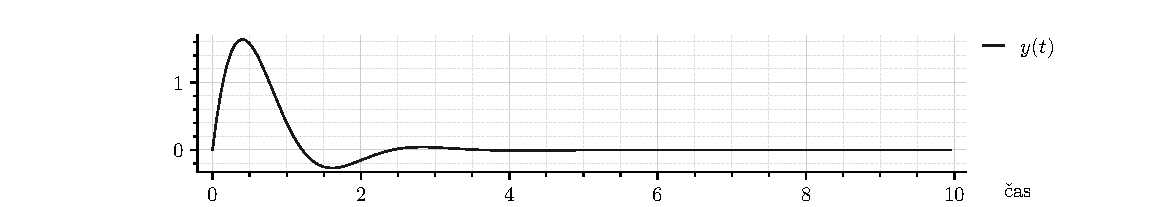
\includegraphics{ICH_SS2R_v3_p1.pdf}
        }

        \figcaption{Graf funkcie \eqref{fun_ICH_SS2R_v3}}
        \label{ICH_SS2R_v3_p1}
    }%vbox

\end{center}




\subsubsection{ICH SS2R, prípad $B(s) = b_1 s + b_0$ alebo  $B(s) = b_1 s $}

Je zrejmé, že v prípade ak polynóm $B(s)$ je v tvare $B(s) = b_1 s + b_0$ alebo $B(s) = b_1 s$ má to vplyv na dynamiku systému.

Napríklad, pre polynóm $A(s)$ uvažujme situáciu rovnakú ako na obr.~\ref{ICH_SS2R_v1_p1}, teda póly systému sú $p_1 = -1$ a $p_2 = -2$, teda $A(s) = s^2 + 3s + 2$. Polynóm $B(s)$ zvoľme $B(s) = 3 s + 2$. V tomto prípade je nula systému, označme ju $z_1$, v bode $z_1 = -\frac{2}{3}$ a~teda táto nula sa nezhoduje so žiadnym pólom.

Obraz výstupnej veličiny pri Dirackovom impulze na vstupe je
\begin{align}
    Y(s) = \frac{3s + 2}{s^2 + 3s + 2} = \frac{3s + 2}{(s + 1)(s + 2)} = \frac{-1}{s + 1} + \frac{4}{s + 2}
\end{align}
Originál potom je
\begin{align} \label{fun_ICH_SS2R_v4}
    y(t) = -e^{-t} + 4e^{-2t}
\end{align}
\begin{center}

    \vbox{%
        \makebox[\textwidth][c]{%
        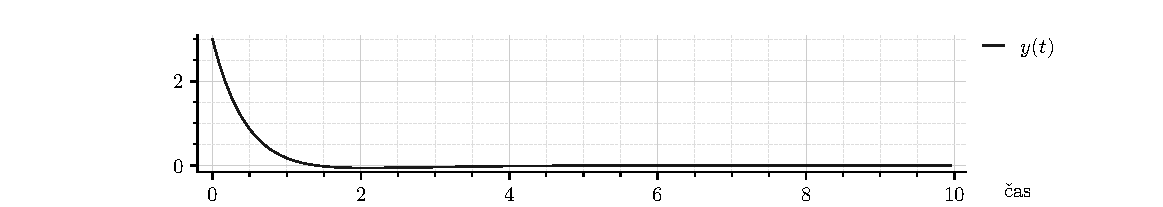
\includegraphics{ICH_SS2R_v4_p1.pdf}
        }

        \figcaption{Graf funkcie \eqref{fun_ICH_SS2R_v4}}
        \label{ICH_SS2R_v4_p1}
    }%vbox

\end{center}

Ak by sa nula zhodovala s pólom, teda napr bola by to $z_1 = -1$, potom by sme mali $G(s) =  \frac{s + 1}{s^2 + 3 s + 2}$, čo je možné zapísať aj ako $G(s) =  \frac{(s + 1)}{(s+1)(s+2)} =  \frac{1}{(s+2)}$, čo je systém prvého rádu.

Pre úplnosť uvažujme tu aj prípad keď $B(s) = b_1 s$. Zvoľme napríklad $b_1 = 3$. Zachovávame $A(s) = s^2 + 3 s + 2$. Všimnime si, že teraz máme $b_0 = 0$. To znamená, že zosilnenie systému, teda hodnota $b_0/a_0$ bude v tomto prípade nulové.

Obraz výstupnej veličiny pri Dirackovom impulze na vstupe je
\begin{align}
    Y(s) = \frac{3s}{s^2 + 3s + 2} = \frac{3s}{(s + 1)(s + 2)} = \frac{-3}{s + 1} + \frac{6}{s + 2}
\end{align}
Originál potom je
\begin{align} \label{fun_ICH_SS2R_v5}
    y(t) = -3e^{-t} + 6e^{-2t}
\end{align}
\begin{center}

    \vbox{%
        \makebox[\textwidth][c]{%
        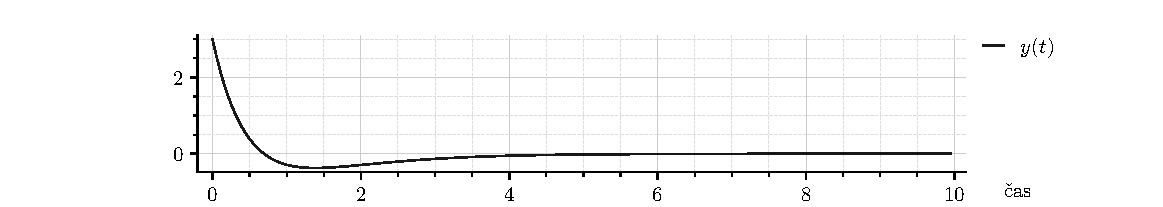
\includegraphics{ICH_SS2R_v5_p1.pdf}
        }

        \figcaption{Graf funkcie \eqref{fun_ICH_SS2R_v5}}
        \label{ICH_SS2R_v5_p1}
    }%vbox

\end{center}

Poznámka: póly systému sme tu zvolili čisto reálne (bez imaginárnej časti) a nie komplexne združené. Je zrejmé, že vplyv nuly na dynamiku systému má charakter kmitania a komplexne združené póly by túto skutočnosť v tejto ukážke zakryli, pretože sami vedú na kmitavú odpoveď systému.


\subsubsection{ICH AS2R}

Ak je jeden z pólov systému nulový, hovoríme, že systém je astatický („obsahuje astatizmus“). Ak práve jeden pól je nulový, hovoríme o astatizme prvého rádu. Zvoľme tu $B(s) = 1$ a póly $p_1 = -1$ a $p_2 = 0$. Teda $A(s) = s^2 + s$.

Obraz výstupnej veličiny pri Dirackovom impulze na vstupe je
\begin{align}
    Y(s) = \frac{1}{s^2 + s} = \frac{1}{s(s + 1)} = \frac{1}{s} - \frac{1}{s + 1}
\end{align}
Originál potom je
\begin{align} \label{fun_ICH_AS2R_v1}
    y(t) = 1 - e^{-t}   
\end{align}
\begin{center}

    \vbox{%
        \makebox[\textwidth][c]{%
        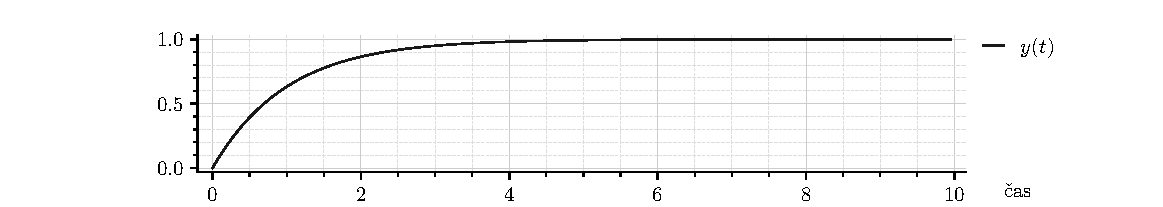
\includegraphics{ICH_AS2R_v1_p1.pdf}
        }

        \figcaption{Graf funkcie \eqref{fun_ICH_AS2R_v1}}
        \label{ICH_AS2R_v1_p1}
    }%vbox

\end{center}

Prípadne by sme mohli mať póly $p_1 = 0$ a $p_2 = 0$. Teda $A(s) = s^2$. Obraz výstupnej veličiny pri Dirackovom impulze na vstupe je
\begin{align}
    Y(s) = \frac{1}{s^2} 
\end{align}
Originál potom je
\begin{align} \label{fun_ICH_AS2R_v2}
    y(t) = t
\end{align}
\begin{center}

    \vbox{%
        \makebox[\textwidth][c]{%
        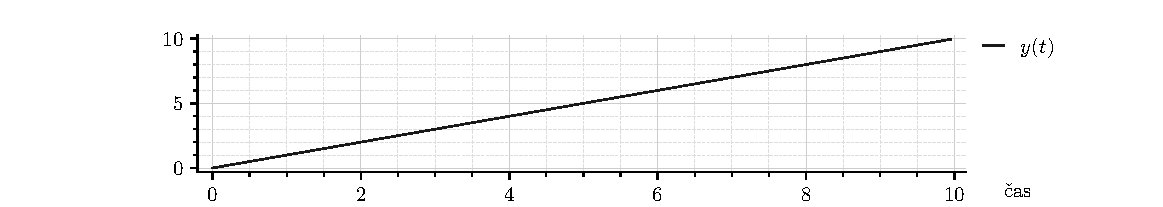
\includegraphics{ICH_AS2R_v2_p1.pdf}
        }

        \figcaption{Graf funkcie \eqref{fun_ICH_AS2R_v2}}
        \label{ICH_AS2R_v2_p1}
    }%vbox

\end{center}

Azda len pre zaujímavosť tu zvoľme $B(s) =  s + 1$, pritom ponechajme póly $p_1 = 0$ a~$p_2 = 0$, teda $A(s) = s^2$. Obraz výstupnej veličiny pri Dirackovom impulze na vstupe je
\begin{align}
    Y(s) = \frac{s + 1}{s^2} = \frac{1}{s} + \frac{1}{s^2}
\end{align}
Originál potom je
\begin{align} \label{fun_ICH_AS2R_v3}
    y(t) = 1 + t
\end{align}
% \begin{center}

%     \vbox{%
%         \makebox[\textwidth][c]{%
%         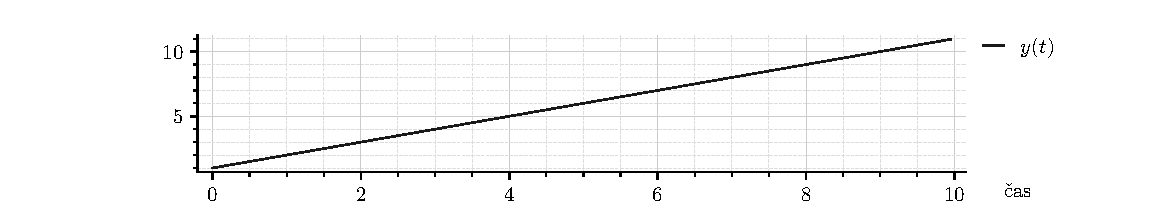
\includegraphics{ICH_AS2R_v3_p1.pdf}
%         }

%         \figcaption{Graf funkcie \eqref{fun_ICH_AS2R_v3}}
%         \label{ICH_AS2R_v3_p1}
%     }%vbox

% \end{center}




\subsection{Prechodová charakteristika}


Prechodová charakteristika je odpoveď systému na jednotkový skok.

Keďže máme k dispozícii matematický opis systému, prechodovú charakteristiku môžeme	nájsť analyticky. Laplaceov obraz jednotkového skoku je $U(s) = \frac{1}{s}$.

\subsubsection{PCH SS2R, prípad $B(s) = b_0$}

V prvom rade uvažujme prípad, keď dynamiku systému určujú len póly systému, teda prenosová funkcia je v tvare
\begin{align}
    G(s) =  \frac{b_0}{s^2 + a_1 s + a_0}
\end{align}

Polynóm $B(s) = b_0$ je nultého stupňa, teda systém nemá žiadne nuly. Označme póly systému $p_1$ a $p_2$. 

\paragraph{Dva nezávislé reálne póly}

Zvoľme prípad, keď sú dva nezávislé reálne póly, teda napr. $p_1 = -1$ a $p_2 = -2$. Parameter $b_0$ zvoľme tak, že statické zosilnenie systému bude jednotkové, teda $b_0 = a_0$. 

Polynóm $A(s)$ je teda $A(s) = \left( s + 1 \right) \left( s + 2 \right) = s^2 + 3s + 2$ a~parameter $b_0 = 2$. Obraz výstupnej veličiny pri jednotkovom skoku na vstupe je
\begin{align}
    Y(s) = \frac{2}{s^2 + 3s + 2} \frac{1}{s} = \frac{2}{(s + 1)(s + 2)} \frac{1}{s} = \frac{1}{s} - \frac{2}{s + 1} + \frac{1}{s + 2}
\end{align}
Originál potom je
\begin{align} \label{fun_PCH_SS2R_v1}
    y(t) = 1 - 2e^{-t} + e^{-2t}
\end{align}
\begin{center}

    \vbox{%
        \makebox[\textwidth][c]{%
        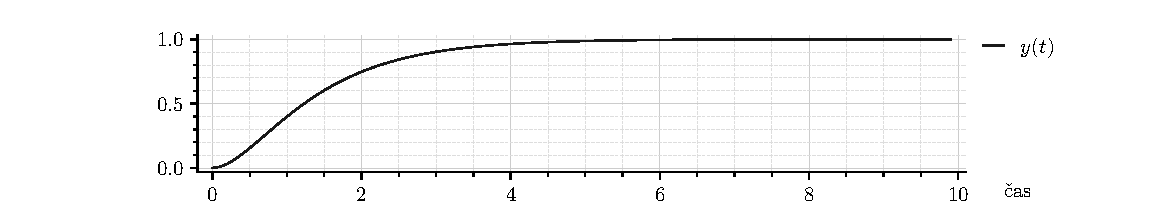
\includegraphics{PCH_SS2R_v1_p1.pdf}
        }

        \figcaption{Graf funkcie \eqref{fun_PCH_SS2R_v1}}
        \label{PCH_SS2R_v1_p1}
    }%vbox

\end{center}



\paragraph{Dva rovnaké reálne póly (jeden dvojnásobný pól)}

Zvoľme prípad, keď sú dva nezávislé reálne póly, teda napr. $p_1 = -1$ a $p_2 = -1$. Parameter $b_0$ zvoľme tak, že statické zosilnenie systému bude jednotkové, teda $b_0 = a_0$. Polynóm $A(s)$ je teda $A(s) = \left( s + 1 \right) \left( s + 1 \right) = s^2 + 2s + 1$ a~parameter $b_0 = 1$. Obraz výstupnej veličiny pri jednotkovom skoku na vstupe je
\begin{align}
    Y(s) = \frac{1}{s^2 + 2s + 1} \frac{1}{s} = \frac{1}{(s + 1)(s + 1)} \frac{1}{s} = \frac{1}{(s + 1)^2} \frac{1}{s} =  \frac{-1}{(s + 1)^2} + \frac{-1}{s + 1} + \frac{1}{s}
\end{align}
Originál je
\begin{align} \label{fun_PCH_SS2R_v2}
    y(t) = -te^{-t} - e^{-t} + 1
\end{align}
\begin{center}

    \vbox{%
        \makebox[\textwidth][c]{%
        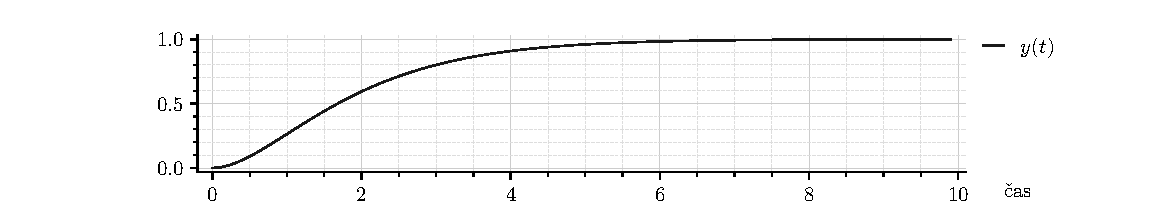
\includegraphics{PCH_SS2R_v2_p1.pdf}
        }

        \figcaption{Graf funkcie \eqref{fun_PCH_SS2R_v2}}
        \label{PCH_SS2R_v2_p1}
    }%vbox

\end{center}

\paragraph{Dva komplexne združené póly}

Ak by sme chceli póly systému, ktoré sú navzájom komplexne združenými číslami, potom je v prípade systému druhého rádu výhodné uvažovať charakteristický polynóm v tvare
\begin{align}
    A(s) = s^2 + 2 \beta \omega_0 s + \omega_0^2
\end{align}
kde $\beta$ a $\omega_0$ sú parametre, pričom $\beta$ sa nazýva koeficient tlmenia a $\omega_0$ sa nazýva vlastná frekvencia systému.

Zvoľme $\beta = 0,5$ a $\omega_0 = 3$. Polynóm $A(s)$ je teda $A(s) = s^2 + 3s + 9 = \left( s + \frac{3}{2} + \frac{3}{2} \sqrt{3} j \right) \left( s + \frac{3}{2} - \frac{3}{2} \sqrt{3} j \right) $. Parameter $b_0$ zvoľme tak, že statické zosilnenie systému bude jednotkové, teda $b_0 = 9$. Obraz výstupnej veličiny pri jednotkovom skoku na vstupe je
\begin{align}
    \begin{aligned}
        Y(s) &= \frac{9}{s^2 + 3s + 9} \frac{1}{s} 
    \end{aligned}
\end{align}
Originál je
\begin{align} \label{fun_PCH_SS2R_v3} 
    1-{{e}}^{-\frac{3\,t}{2}}\,\left(\cos\left(\frac{3\,\sqrt{3}\,t}{2}\right)+\frac{\sqrt{3}\,\sin\left(\frac{3\,\sqrt{3}\,t}{2}\right)}{3}\right)
\end{align}
čo bolo v tomto prípade určené s využitím \lstinline|Symbolic Math Toolbox| v~MATLAB-e ako ukazuje nasledujúci výpis kódu.
\begin{center}

    \vbox{%
        \makebox[\textwidth][c]{%
        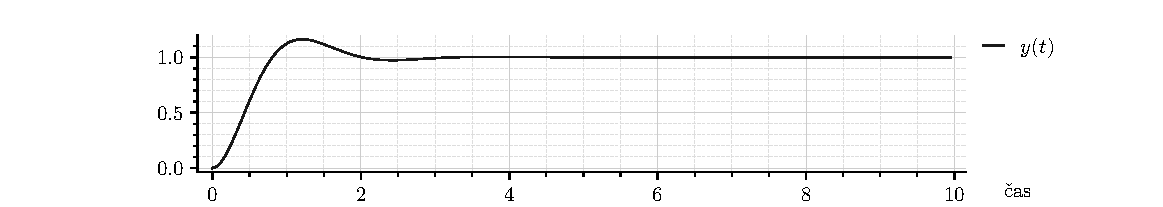
\includegraphics{PCH_SS2R_v3_p1.pdf}
        }

        \figcaption{Graf funkcie \eqref{fun_PCH_SS2R_v2}}
        \label{PCH_SS2R_v3_p1}
    }%vbox

\end{center}


% % python jupynotex.py ../MRS10_PCH2R_ML.ipynb '5' '70'
\input{../../PY/jupynotex/tex/MRS10_PCH2R_MLipynb_5.tex}



\subsubsection{PCH SS2R, prípad $B(s) = b_1 s + b_0$ alebo  $B(s) = b_1 s $}

Je zrejmé, že v prípade ak polynóm $B(s)$ je v tvare $B(s) = b_1 s + b_0$ alebo $B(s) = b_1 s$ má to vplyv na dynamiku systému.

Napríklad, pre polynóm $A(s)$ uvažujme situáciu rovnakú ako na obr.~\ref{PCH_SS2R_v1_p1}, teda póly systému sú $p_1 = -1$ a $p_2 = -2$, teda $A(s) = s^2 + 3s + 2$. Polynóm $B(s)$ zvoľme $B(s) = 3 s + 2$. V tomto prípade je nula systému, označme ju $z_1$, v bode $z_1 = -\frac{2}{3}$ a~teda táto nula sa nezhoduje so žiadnym pólom. Obraz výstupnej veličiny pri jednotkovom skoku na vstupe je
\begin{align}
    Y(s) = \frac{3s + 2}{s^2 + 3s + 2} \frac{1}{s} = \frac{3s + 2}{(s + 1)(s + 2)} \frac{1}{s} = \frac{1}{s} + \frac{1}{s + 1} - \frac{2}{s + 2}
\end{align}
Originál je
\begin{align} \label{fun_PCH_SS2R_v4}
    y(t) = 1 + e^{-t} - 2e^{-2t}
\end{align}
\begin{center}

    \vbox{%
        \makebox[\textwidth][c]{%
        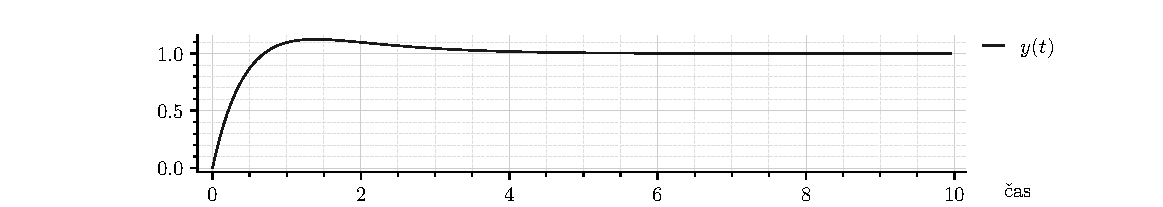
\includegraphics{PCH_SS2R_v4_p1.pdf}
        }

        \figcaption{Graf funkcie \eqref{fun_PCH_SS2R_v4}}
        \label{PCH_SS2R_v4_p1}
    }%vbox

\end{center}

Ak by sa nula zhodovala s pólom, teda napr bola by to $z_1 = -1$, potom by sme mali $G(s) =  \frac{s + 1}{s^2 + 3 s + 2}$, čo je možné zapísať aj ako $G(s) =  \frac{(s + 1)}{(s+1)(s+2)} =  \frac{1}{(s+2)}$, čo je systém prvého rádu.

Pre úplnosť uvažujme tu aj prípad keď $B(s) = b_1 s$. Zvoľme napríklad $b_1 = 3$. Zachovávame $A(s) = s^2 + 3 s + 2$. Všimnime si, že teraz máme $b_0 = 0$. To znamená, že zosilnenie systému, teda hodnota $b_0/a_0$ bude v tomto prípade nulové. Obraz výstupnej veličiny pri jednotkovom skoku na vstupe je
\begin{align}
    Y(s) = \frac{3s}{s^2 + 3s + 2} \frac{1}{s} = \frac{3s}{(s + 1)(s + 2)} \frac{1}{s} =  \frac{3}{s + 1} - \frac{3}{s + 2}
\end{align}
Originál je
\begin{align} \label{fun_PCH_SS2R_v5}
    y(t) = 3e^{-t} - 3e^{-2t}
\end{align}
\begin{center}

    \vbox{%
        \makebox[\textwidth][c]{%
        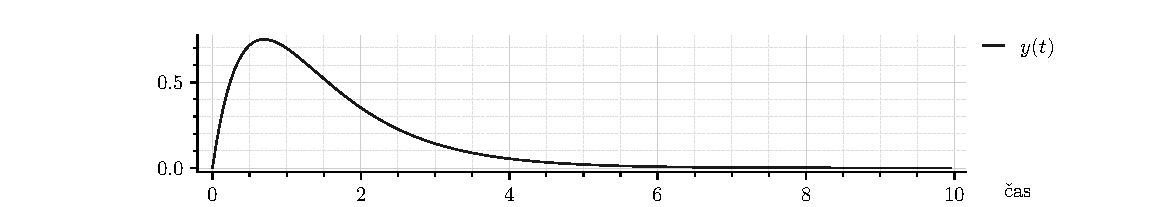
\includegraphics{PCH_SS2R_v5_p1.pdf}
        }

        \figcaption{Graf funkcie \eqref{fun_PCH_SS2R_v5}}
        \label{PCH_SS2R_v5_p1}
    }%vbox

\end{center}

Poznámka: póly systému sme tu zvolili čisto reálne (bez imaginárnej časti) a nie komplexne združené. Je zrejmé, že vplyv nuly na dynamiku systému má charakter kmitania a komplexne združené póly by túto skutočnosť v tejto ukážke zakryli, pretože sami vedú na kmitavú odpoveď systému.


\subsubsection{PCH AS2R}

Ak je jeden z pólov systému nulový, hovoríme, že systém je astatický („obsahuje astatizmus“). Ak práve jeden pól je nulový, hovoríme o astatizme prvého rádu. Zvoľme tu $B(s) = 1$ a póly $p_1 = -1$ a $p_2 = 0$. Teda $A(s) = s^2 + s$. Obraz výstupnej veličiny pri jednotkovom skoku na vstupe je
\begin{align}
    Y(s) = \frac{1}{s^2 + s} \frac{1}{s} = \frac{1}{s(s + 1)} \frac{1}{s} = \frac{1}{s^2} - \frac{1}{s} + \frac{1}{s+1} 
\end{align}
Originál je
\begin{align} \label{fun_PCH_AS2R_v1}
    y(t) = t - 1 + e^{-t}
\end{align}
\begin{center}

    \vbox{%
        \makebox[\textwidth][c]{%
        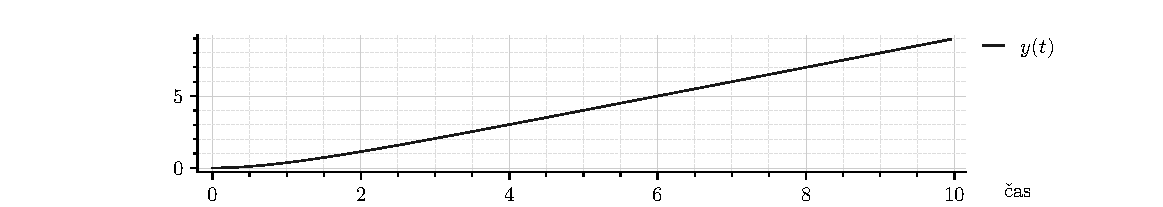
\includegraphics{PCH_AS2R_v1_p1.pdf}
        }

        \figcaption{Graf funkcie \eqref{fun_PCH_AS2R_v1}}
        \label{PCH_AS2R_v1_p1}
    }%vbox

\end{center}

Prípadne by sme mohli mať póly $p_1 = 0$ a $p_2 = 0$. Teda $A(s) = s^2$. Obraz výstupnej veličiny pri jednotkovom skoku na vstupe je
\begin{align}
    Y(s) = \frac{1}{s^2} \frac{1}{s} = \frac{1}{s^3}
\end{align}
Originál je
\begin{align} \label{fun_PCH_AS2R_v2}
    y(t) = \frac{t^2}{2}
\end{align}
\begin{center}

    \vbox{%
        \makebox[\textwidth][c]{%
        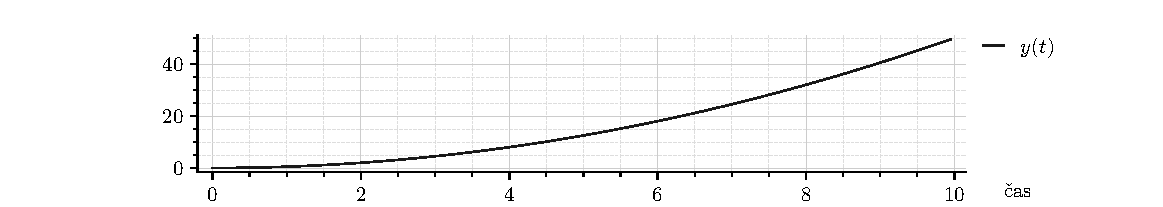
\includegraphics{PCH_AS2R_v2_p1.pdf}
        }

        \figcaption{Graf funkcie \eqref{fun_PCH_AS2R_v2}}
        \label{PCH_AS2R_v2_p1}
    }%vbox

\end{center}

Azda len pre zaujímavosť tu zvoľme $B(s) =  s + 1$, pritom ponechajme póly $p_1 = 0$ a~$p_2 = 0$, teda $A(s) = s^2$. Obraz výstupnej veličiny pri jednotkovom skoku na vstupe je
\begin{align}
    Y(s) = \frac{s + 1}{s^2} \frac{1}{s} = \frac{s + 1}{s^3} = \frac{1}{s^3} + \frac{1}{s^2}
\end{align}
Originál je
\begin{align} \label{fun_PCH_AS2R_v3}
    y(t) = \frac{t^2}{2} + t
\end{align}
% \begin{center}

%     \vbox{%
%         \makebox[\textwidth][c]{%
%         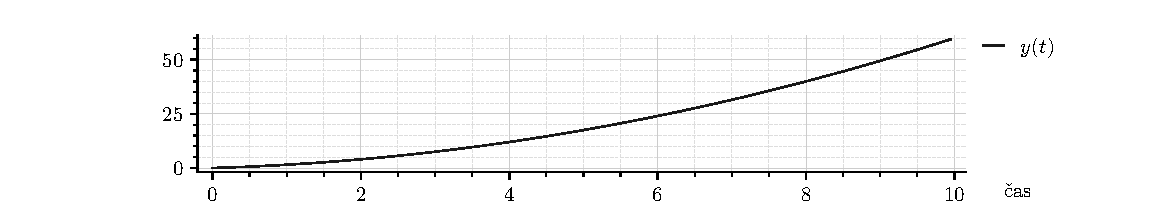
\includegraphics{PCH_AS2R_v3_p1.pdf}
%         }

%         \figcaption{Graf funkcie \eqref{fun_PCH_AS2R_v3}}
%         \label{PCH_AS2R_v3_p1}
%     }%vbox

% \end{center}













\section{Doplnkové úlohy na cvičenia}

Priestor pre oboznámenie sa s typickým „control toolboxom“ - sadou výpočtových nástrojov pre oblasť návrhu riadiacich systémov (napr. Control System Toolbox v~MATLABe).

\subsection*{Úlohy}

\begin{enumerate}[leftmargin=0pt, labelsep=4mm, itemsep=0pt]

	\item Vypočítajte póly lineárnych dynamických systémov daných prenosovými funkciami.
	
	\item Nakreslite prechodové charakteristiky lineárnych dynamických systémov daných prenosovými funkciami.

    \item Nakreslite impulzné charakteristiky lineárnych dynamických systémov daných prenosovými funkciami.
    
\end{enumerate}


\noindent
Lineárne dynamické systémy sú pre tieto úlohy definované prenosovou funkciou so všeobecnými parametrami v tvare
\begin{equation*}
	G(s) = \frac{b_2 s^2 + b_1 s + b_0}{a_3 s^3 + a_2 s^2 + a_1 s + a_0} e^{-Ds}
\end{equation*}
a tabuľkou, v ktorej sú uvedené hodnoty parametrov jednotlivých systémov:



\bigskip




\begin{centering}
\catcode`\-=12

\begin{tabular*}{1.0\columnwidth}{ @{\extracolsep{\fill}} c  c c c c c c c c c c }
\toprule
\multicolumn{1}{l}{Systém} & \multicolumn{8}{l}{Parameter} & \multicolumn{1}{l}{Obrázok}   \\
 & $b_2$ & $b_1$ & $b_0$ & $a_3$ & $a_2$ & $a_1$ & $a_0$ & $D$ & \multicolumn{1}{c}{PCH}    \\
\midrule
$1$. & & & $1$ & & & $1$ & $1$ & & \multirow{4}{*}[-6pt]{\rotatebox{90}{Obr. 1.}}   \\
$2$. & & & $1$ & & & $1$ & $1$ & $5$ &   \\
$3$. & & & $0,1$ & & & $1$ & $0$ & &   \\
$4$. & & & $0,1$ & & & $1$ & $0$ & $3$ &   \\ \cmidrule{10-10}
$5$. & & $1$ & $1$ & & & $3$ & $1$ & & \multirow{2}{*}[0pt]{\rotatebox{90}{2.}}  \\
$6$. & & $1$ & $-1$ & & & $3$ & $1$ & & & \\ \cmidrule{10-10}
$7$. & & & $0,5$ & & $1$ & $2$ & $1$ & &  \multirow{4}{*}[0pt]{\rotatebox{90}{Obr. 3.}}  \\
$8$. & & & $0,5$ & & $1$ & $1$ & $1$ & & & \\
$9$. & & & $0,5$ & & $1$ & $0,2$ & $1$ & & & \\
$10$. & & & $0,5$ & & $1$ & $0$ & $1$ & &  & \\ \cmidrule{10-10}
$11$. & & & $0,2$ & & $1$ & $1$ & $0$ & & \multirow{3}{*}[-3pt]{\rotatebox{90}{Obr. 4.}}   \\
$12$. & & & $0,2$ & & $1$ & $0$ & $0$ & &   \\
$13$. & & & $0,2$ & & $1$ & $0$ & $0$ & $4$ &   \\ \cmidrule{10-10}
$14$. & $1$ & $2$ & $2$ & $1$ & $0,3$ & $4,03$ & $0,401$ &  & \multirow{2}{*}[0pt]{\rotatebox{90}{5.}}   \\
$15$. & $1$ & $2$ & $2$ & $1$ & $0,3$ & $4,03$ & $0,401$ & $6$ &  \\
\bottomrule
\end{tabular*}
\end{centering}

\medskip

\noindent
Tabuľka určuje aj číslo obrázka, do ktorého nakreslite príslušnú charakteristiku (PCH). Niektoré charakteristiky sú na spoločnom obrázku.

















\section{Otázky a úlohy}


\begin{enumerate}[leftmargin=0pt, labelsep=3mm, itemsep=0pt]

    \item Definujte prenosovú funkciu systému.

    \item Ako sa nazýva pomer Laplaceovho obrazu výstupného signálu systému k~Laplaceovmu obrazu vstupného signálu systému pri nulových začiatočných podmienkach systému?





    \item Nájdite prenosovú funkciu dynamického systému daného diferenciálnou rovicou v~tvare
    \begin{align*}
        a_1 \dot y(t) + a_0 y(t) = b_0 u(t) \qquad a_0, a_1, b_0\in\mathbb R
    \end{align*}

    \item Nájdite prenosovú funkciu dynamického systému daného diferenciálnou rovnicou v~tvare
    \begin{align*}
        \ddot y(t) + a_1 \dot y(t) + a_0 y(t) = b_0 u(t) \qquad a_0, a_1, b_0\in\mathbb R
    \end{align*}



    \item Pre dynamický systém opísaný pomocou prenosovej funkcie nájdite zodpovedajúcu diferenciálnu rovnicu.
    \begin{align*}
        G(s) &= \frac{b_0}{s^2 + a_1 s + a_0}
    \end{align*}


    \item Pre dynamický systém opísaný pomocou prenosovej funkcie nájdite zodpovedajúcu diferenciálnu rovnicu.
    \begin{align*}
        G(s) &= \frac{b_1 s}{s^2 + a_1 s + a_0}
    \end{align*}

    \item Určte charakteristický polynóm prenosovej funkcie
    \begin{equation*}
        G(s) = \frac{b_2 s^2 + b_1 s + b_0}{a_3 s^3 + a_2 s^2 + a_1 s + a_0}
    \end{equation*}


    \item Určte póly dynamického systému daného prenosovou funkciou
    \begin{equation*}
        G(s) = \frac{a s + b}{s^2 + (c+d) s + cd}
    \end{equation*}


    \item Vyšetrite stabilitu dynamického systému daného prenosovou funkciou
    \begin{equation*}
        G(s) = \frac{5 s }{s^2 + 5 s + 6}
    \end{equation*}

    \item Nájdite hodnoty koeficientov $a$ a $b$, pre ktoré je dynamický systém stabilný
    \begin{equation*}
        G(s) = \frac{1}{s^2 + (a+b) s + ab}
    \end{equation*}


    \item Určte ustálenú hodnotu (konečnú hodnotu), na ktorej sa ustáli výstup systému daného prenosovou funkciou
    \begin{align*}
        G(s) = \frac{b_0}{s + a_0}
    \end{align*}
    keď vstupom systému je jednotkový skok.


    \item Určte rád astatizmu dynamického systému daného prenosovou funkciou
    \begin{equation*}
        G(s) = \frac{b_0}{s^2 + a_0 s}
    \end{equation*}



    \item Dynamický systém daný prenosovou funkciu prepíšte do opisu v stavovom priestore (stanovte stavové veličiny).
    \begin{align*}
        G(s) = \frac{b_0}{s^2 + a_1 s + a_0}
    \end{align*}

    \item Načrtnite prechodovú charakteristiku statického systému prvého rádu.

    \item Načrtnite prechodovú charakteristiku astatického systému prvého rádu.

    \item Načrtnite prechodovú charakteristiku statického systému druhého rádu, ktorého charakteristický polynóm je v tvare $A(s) = s^2 + 2 \beta \omega_0 s + \omega_0^2$ pričom $\beta = 0$.



\end{enumerate}









% \printbibliography[title={Literatúra}]




% % python .\jupynotex.py ..\MRS10_ICH2R.ipynb '3-' '70'

% \input{../../PY/jupynotex/tex/MRS10_ICH2Ripynb_3-4.tex}




\end{document}
